\documentclass{article}
\usepackage{graphicx} % Required for inserting images
\usepackage{float} % Include the float package
\title{IMMAGINI E RIFLESSIONI TESI}
\author{bignozzi.1855163 }
\date{September 2024}

\begin{document}

\maketitle

\section{GRAFO}
Allora la scelta per il grafo, per semplicità di scrittura è stato quello di fare dei legami solo e solo se il raggio di interazione è minor edi un certo valore. Come si fa a trovare la teshold migliroe per il raggio in quesot modello?
Si runna il modello al fine di minimizzare i MAE sui residui ogni volta ocn un raggio diverso. Il modello che ottiene il mae min,ore è quello che meglio descrive il tutto.
Inoltre in questo modo è possibile ottenre anche il miglior grafo senza alcun tipo di vincolo.
Prima di predirre i beta factor per davvero (con autovalori e autovettori) avrei bisogno di utilizzare i parametri corretti epr temperatura Kb ecc.

\section{Matrice di kirchoff}
La matrice di Kirchhoff (o laplaciana) rappresenta un'analogia con una rete elastica in cui le connessioni tra i nodi (atomi) descrivono le interazioni elastiche. Questa matrice codifica il modo in cui ogni nodo è collegato agli altri, e attraverso i suoi autovalori e autovettori, si può studiare come le vibrazioni collettive (modi normali) si propagano attraverso il sistema.
Autovalori e autovettori della matrice di Kirchhoff:
Gli autovalori della matrice di Kirchhoff descrivono le frequenze naturali di vibrazione del sistema.
Gli autovettori rappresentano i corrispondenti modi normali di vibrazione, cioè come ogni nodo (atomo) si muove in un determinato modo di vibrazione.
Quelli a bassa frequenza corrispondono alle vibrazioni collettive del sistema, quelli ad alta frequenza sono fluttuazioni locali 
% Inserisci la prima immagine
\section{Calcolo correlazione}
Risolvi l'equazione differenziale:
\begin{equation}
    \gamma \dot{x}_i = -g \sum_j K_{ij} x_j + \sqrt{2 \gamma k_B T} \xi_i(t)
    \end{equation}
    
\begin{equation}
    \mathbf{x}(t) = e^{-\mu K t} \left\{ \mathbf{x}(0) + \sqrt{\frac{2k_B T}{\gamma}} \int_0^t ds \, e^{-\mu K s} \xi(s) \right\}
    \end{equation}
\begin{equation}
    C(t) = \langle \mathbf{x}(0) \mathbf{x}^\top(t) \rangle
    \end{equation}
\begin{equation}
    C(t) = e^{-\mu \mathbf{K} t} C(0)
    \end{equation}
        
\begin{equation}
    C(0) = \langle \mathbf{x}(0) \mathbf{x}^\top(0) \rangle
    \end{equation}
\begin{equation}
    \mathbf{K} = \mathbf{U} \Lambda \mathbf{U}^\dagger
    \end{equation}
        
\begin{equation}
    C_{ij}(t) = \frac{3 k_B T}{g} \sum_{k=2}^{N} \frac{u_i(k) u_j(k)}{\lambda(k)} e^{-\lambda(k) t}
    \end{equation}
        
\section{Calcolo risposta}
\begin{equation}
    R(t) = \frac{C(t)}{C(0)}
    \end{equation}
\begin{equation}
    \mathbf{R}(t) = e^{-\mu \mathbf{K} t}
    \end{equation}
\begin{equation}
    R_{ij}(t) = - \left\langle \frac{\partial \ln P_s(x)}{\partial x_j(t)} x_i(0) \right\rangle
    \end{equation}
\begin{equation}
    R_{ij}(t) = \sum_{k=1}^{N} u_i(k) u_j(k) e^{-\lambda(k) t}
    \end{equation}


\section{Cross-Entropy}
\begin{equation}
    TE_{j \rightarrow i}(t) = \left\langle \log \frac{P[x_i(t) | x_i(0), x_j(0)]}{P[x_i(t) | x_i(0)]} \right\rangle
    \end{equation}
        
\begin{equation}
    T_{j \rightarrow i}(t) = - \frac{1}{2} \ln \left( 1 - \frac{\alpha_{ij}(t)}{\beta_{ij}(t)} \right)
    \end{equation}
\begin{equation}
    \alpha_{ij}(t) = [C_{ii}(0) C_{ij}(t) - C_{ij}(0) C_{ii}(t)]^2
    \end{equation}
        


\section{2M0Z}
\begin{figure}[H]
    \centering
    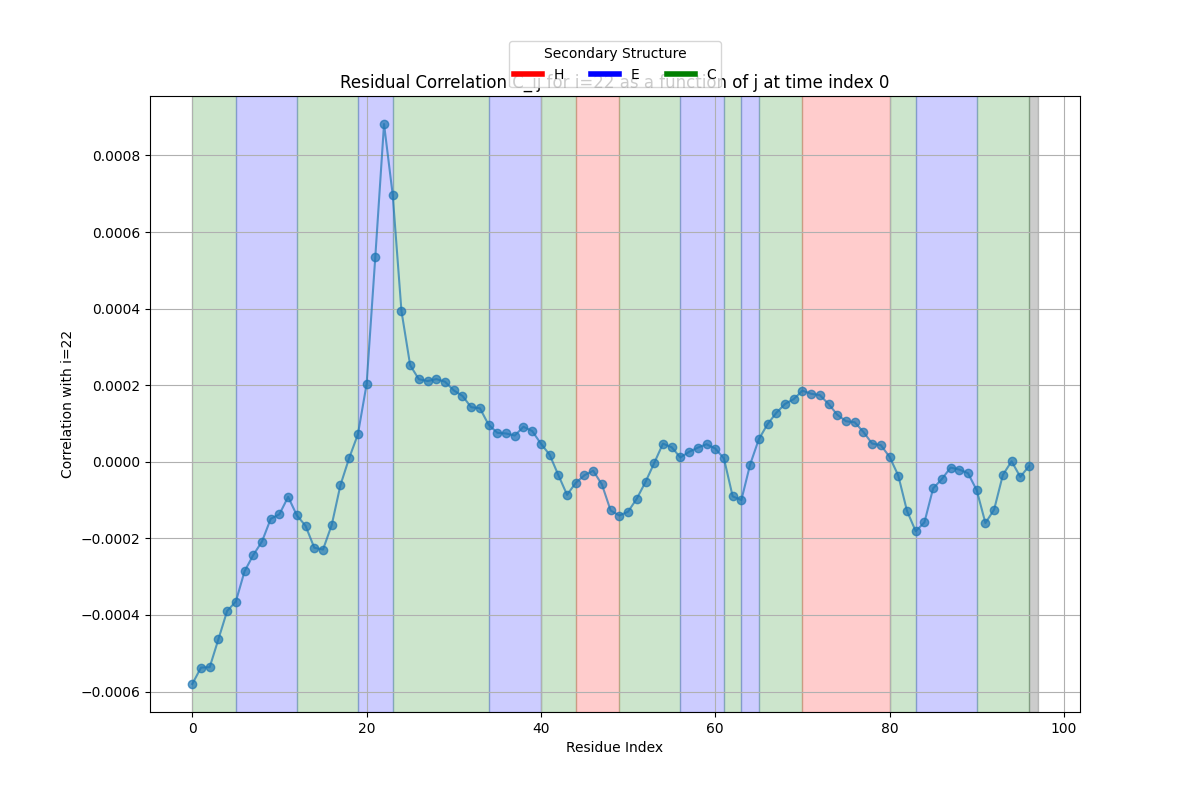
\includegraphics[width=0.5\textwidth]{images/2m0zResidual Correlation C_ij for i=22 as a function of j at time index 0.png}
    \caption{Correlazione}
\end{figure}
\begin{figure}[H]
    \centering
    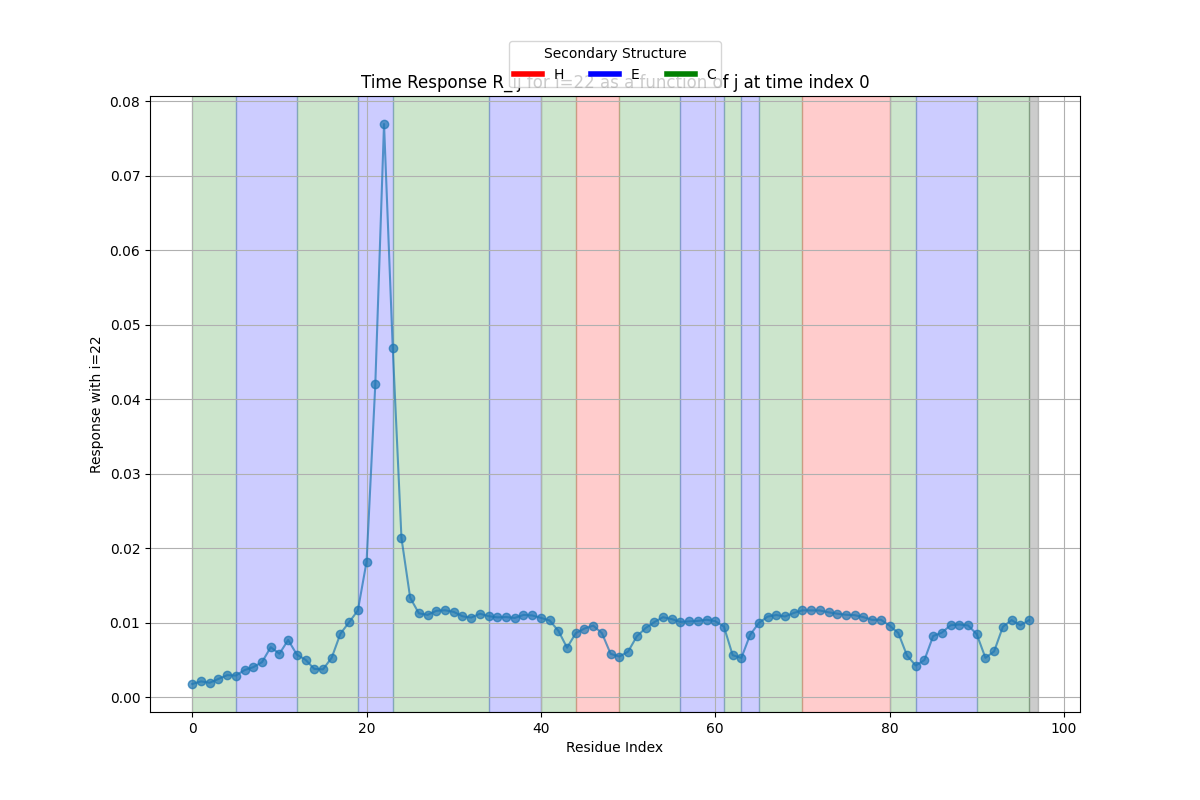
\includegraphics[width=0.5\textwidth]{"images/2m0zTime Response R_ij for i=22 as a function of j at time index 0.png"}
    \caption{Risposta}
\end{figure}

\begin{figure}[H]
    \centering
    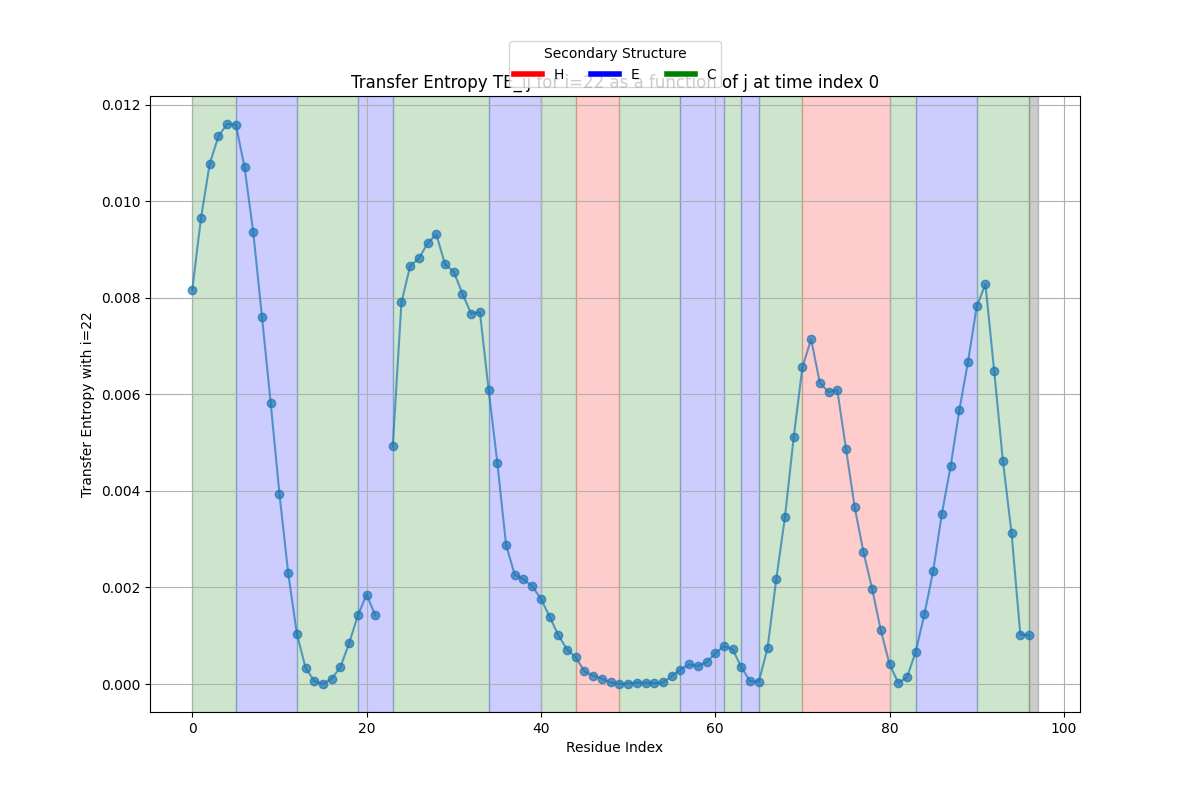
\includegraphics[width=0.5\textwidth]{"images/2m0zTransfer Entropy TE_ij for i=22 as a function of j at time index 0.png"}
    \caption{Transfer Entropy}
\end{figure}
\begin{figure}[H]
    \centering
    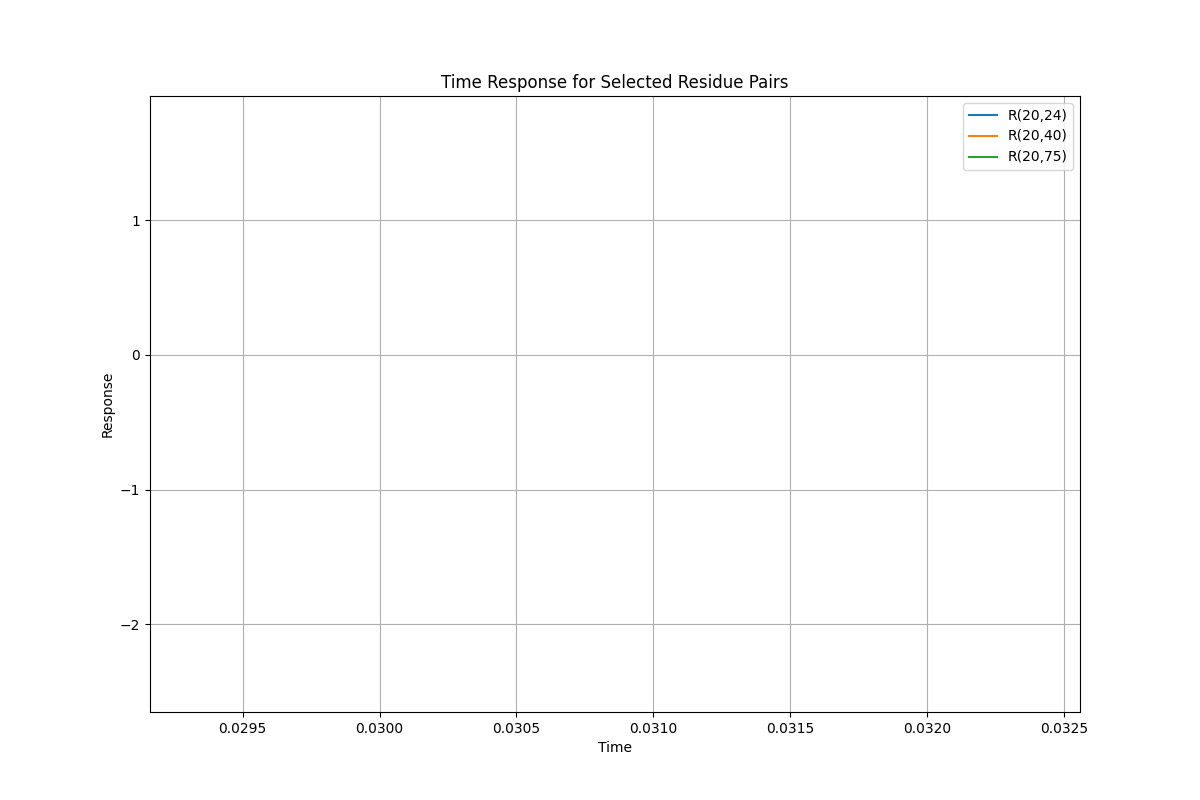
\includegraphics[width=0.5\textwidth]{"images/2m0zMultiple_time_resposne.png"}
    \caption{Multiple time response}
\end{figure}

\begin{figure}[H]
    \centering
    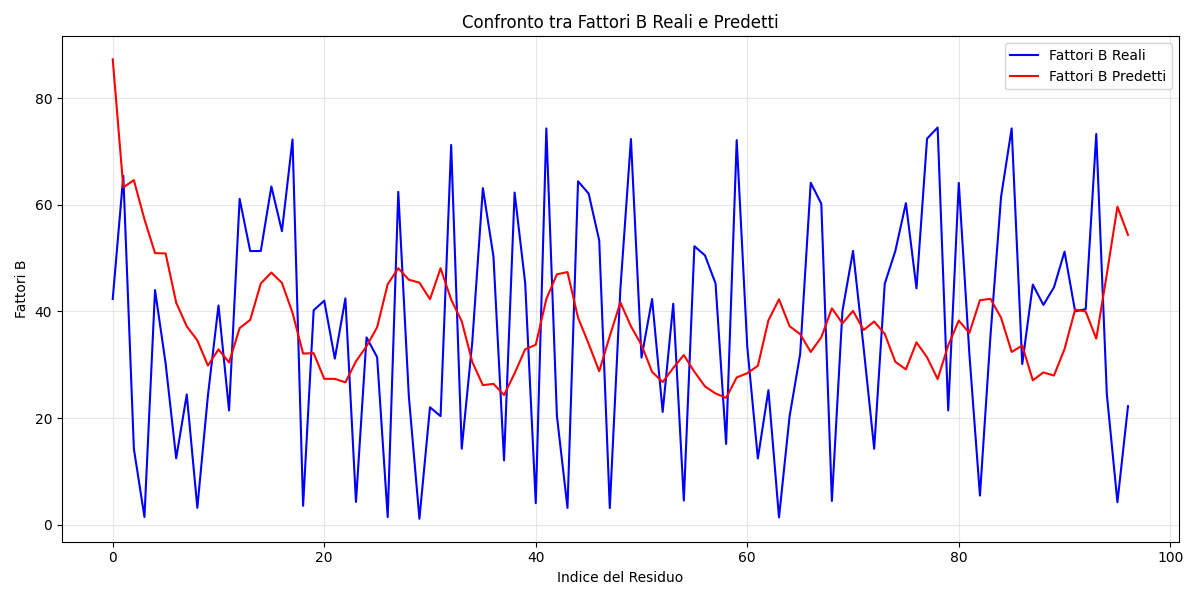
\includegraphics[width=0.5\textwidth]{"images/2m0zConfronto tra Fattori B Reali e Predetti.png"}
    \caption{B factors}
\end{figure}
\begin{figure}[H]
    \centering
    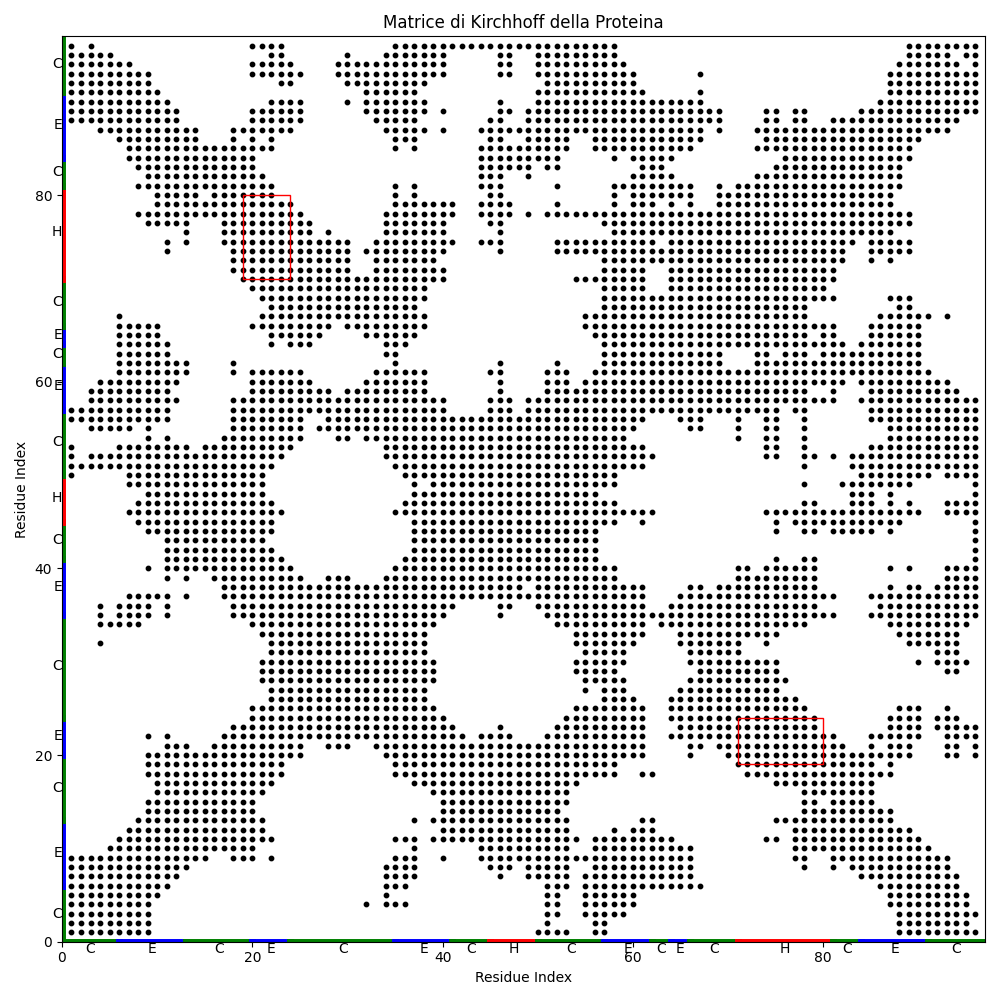
\includegraphics[width=0.5\textwidth]{"images/2m0z_Matrice di Kirchhoff della Proteina.png"}
    \caption{Kirchhoff}
\end{figure}
\begin{figure}[H]
    \centering
    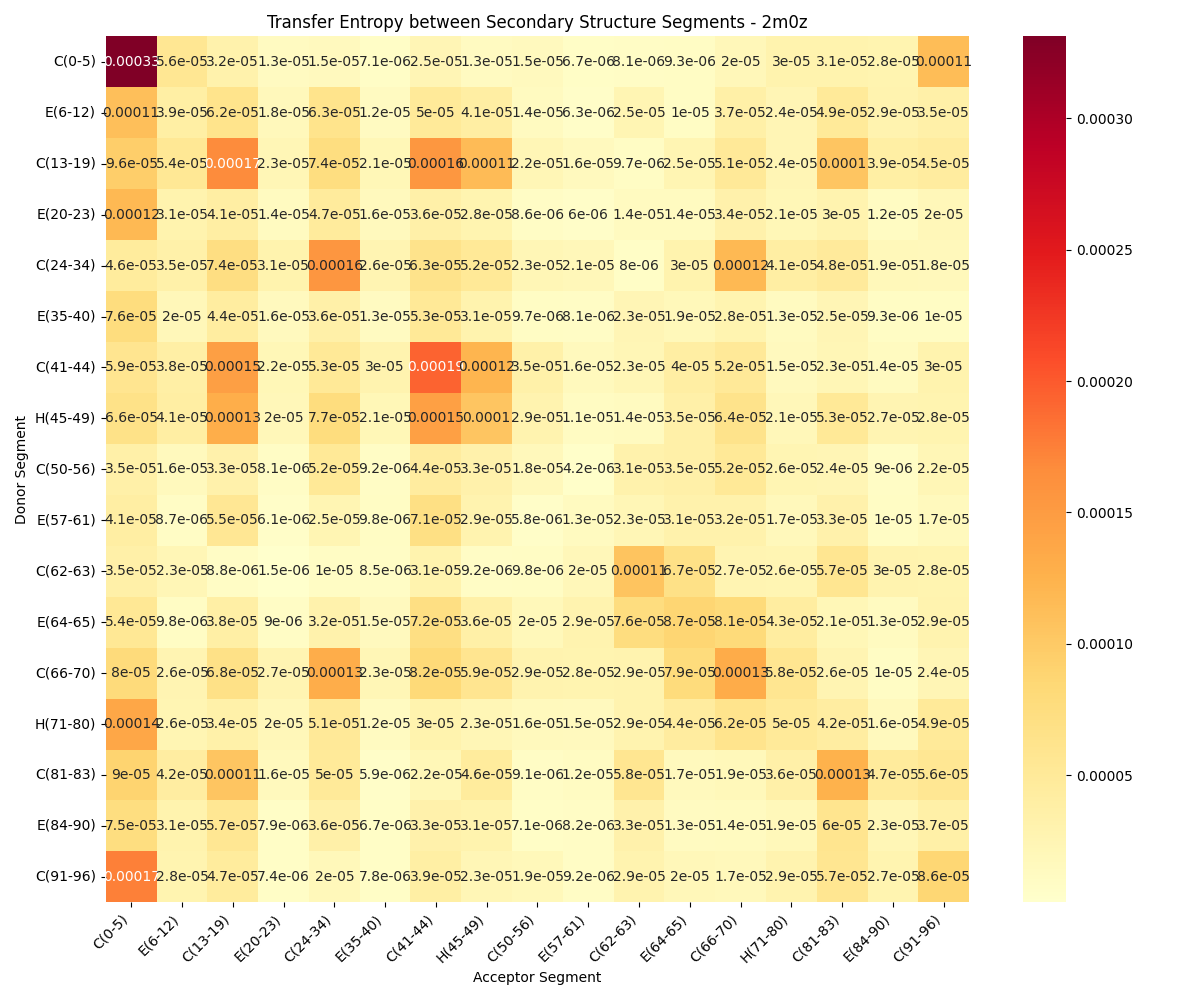
\includegraphics[width=0.5\textwidth]{"images/2m0zanalyze_secondary_structure_transfer_entropy.png"}
    \caption{Secodnaria Structure}
\end{figure}
\section{2M10}
\begin{figure}[H]
    \centering                            
    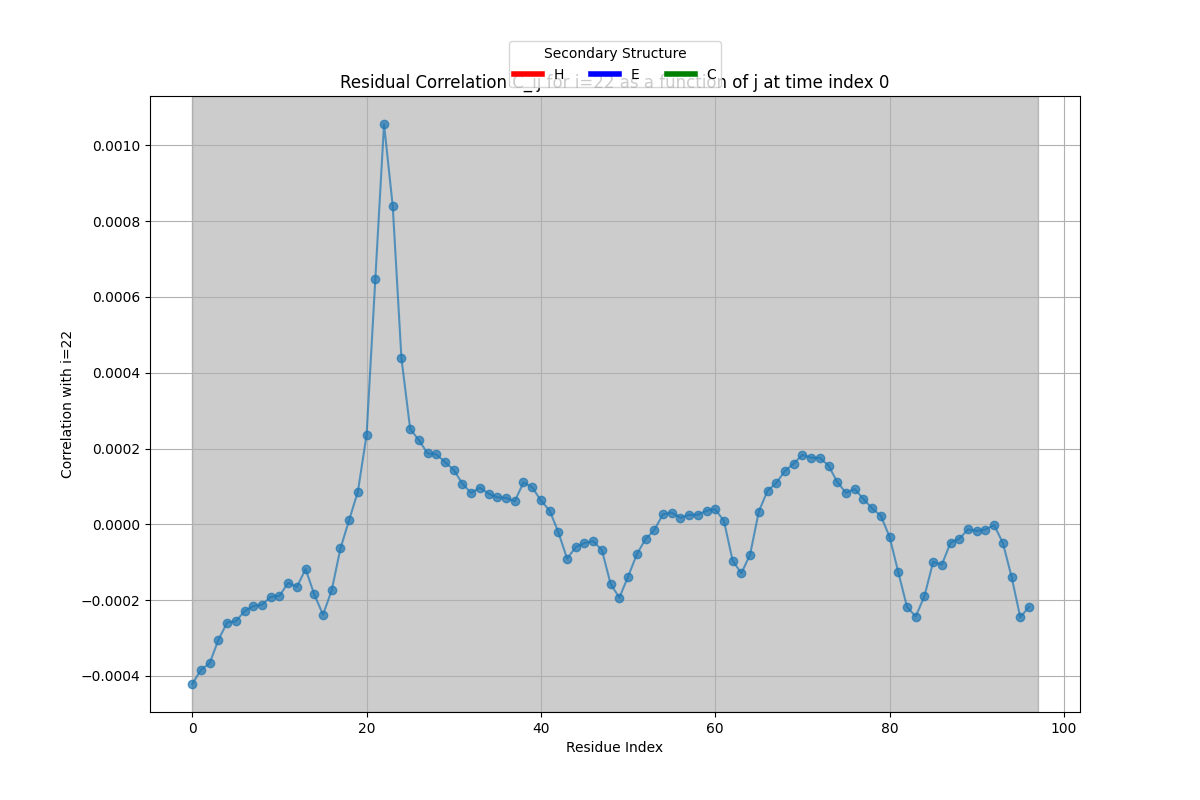
\includegraphics[width=0.5\textwidth]{"images/2m10Residual Correlation C_ij for i=22 as a function of j at time index 0.png"}
    \caption{Correlazione}
\end{figure}
\begin{figure}[H]
    \centering
    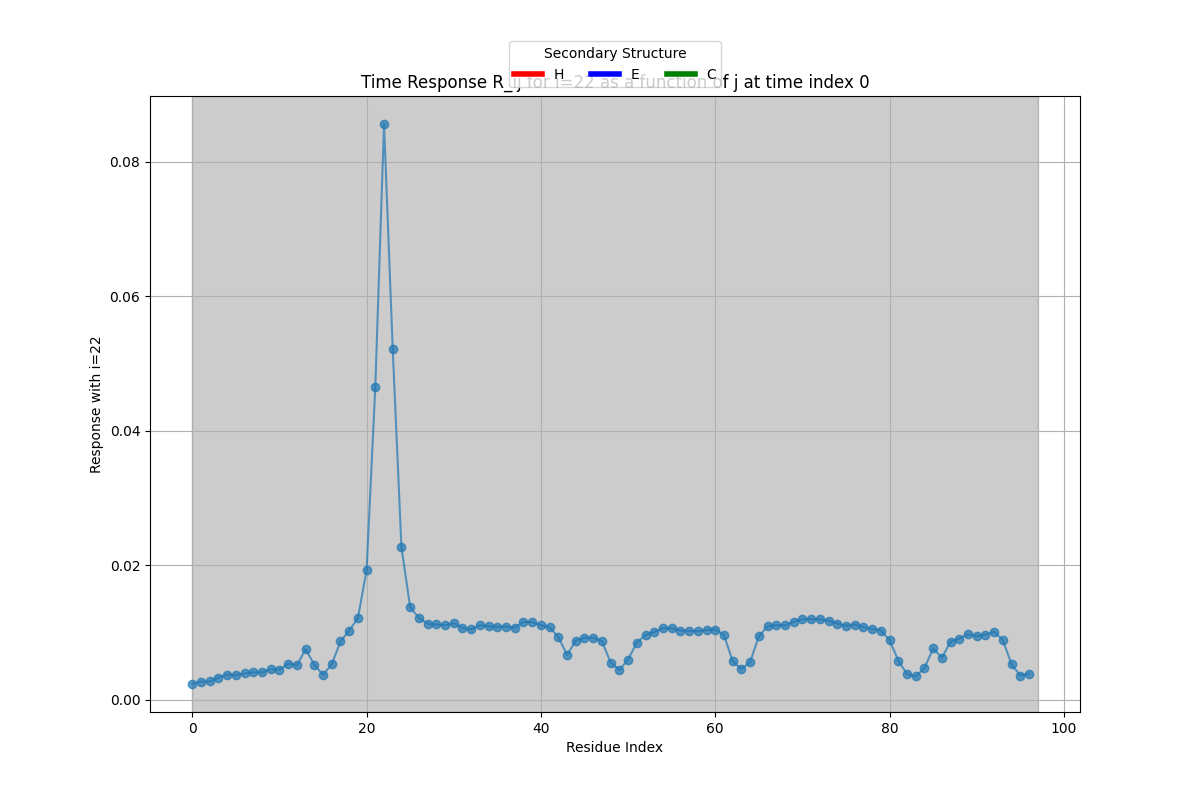
\includegraphics[width=0.5\textwidth]{"images/2m10Time Response R_ij for i=22 as a function of j at time index 0.png"}
    \caption{Risposta}
\end{figure}

\begin{figure}[H]
    \centering
    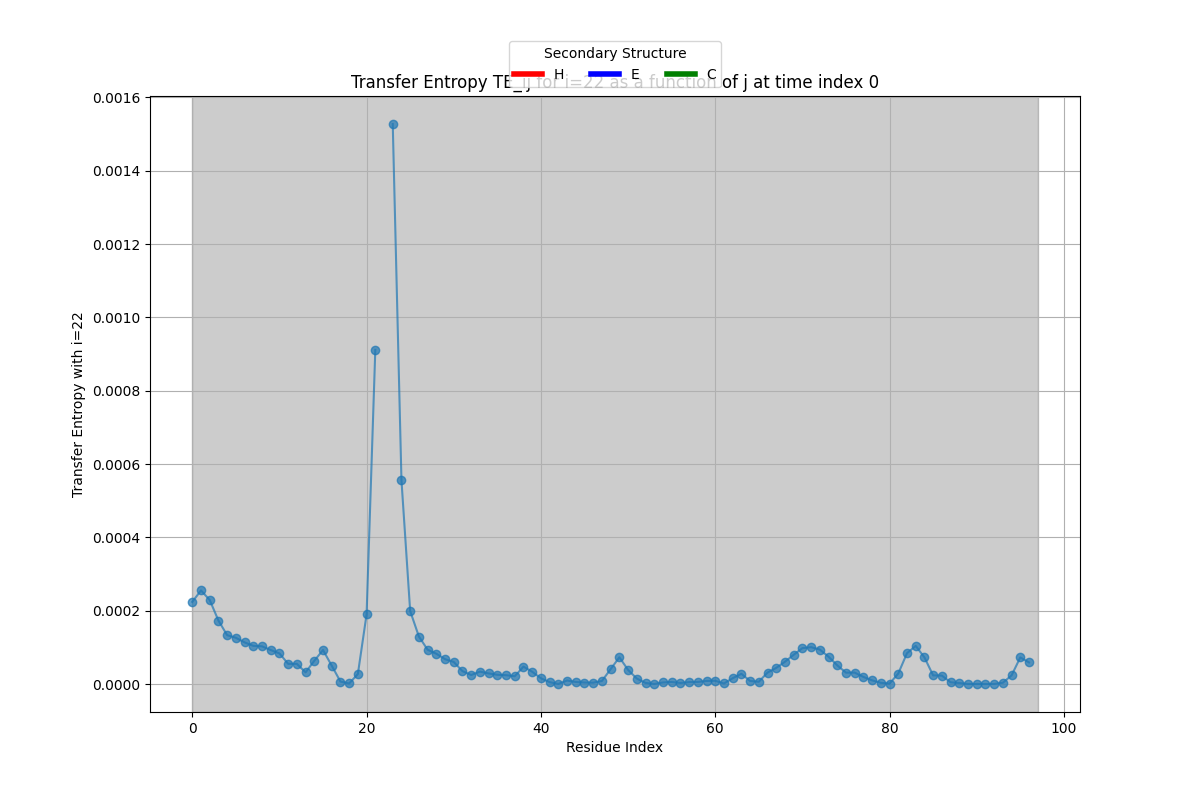
\includegraphics[width=0.5\textwidth]{"images/2m10Transfer Entropy TE_ij for i=22 as a function of j at time index 0.png"}
    \caption{Transfer Entropy}
\end{figure}
\begin{figure}[H]
    \centering
    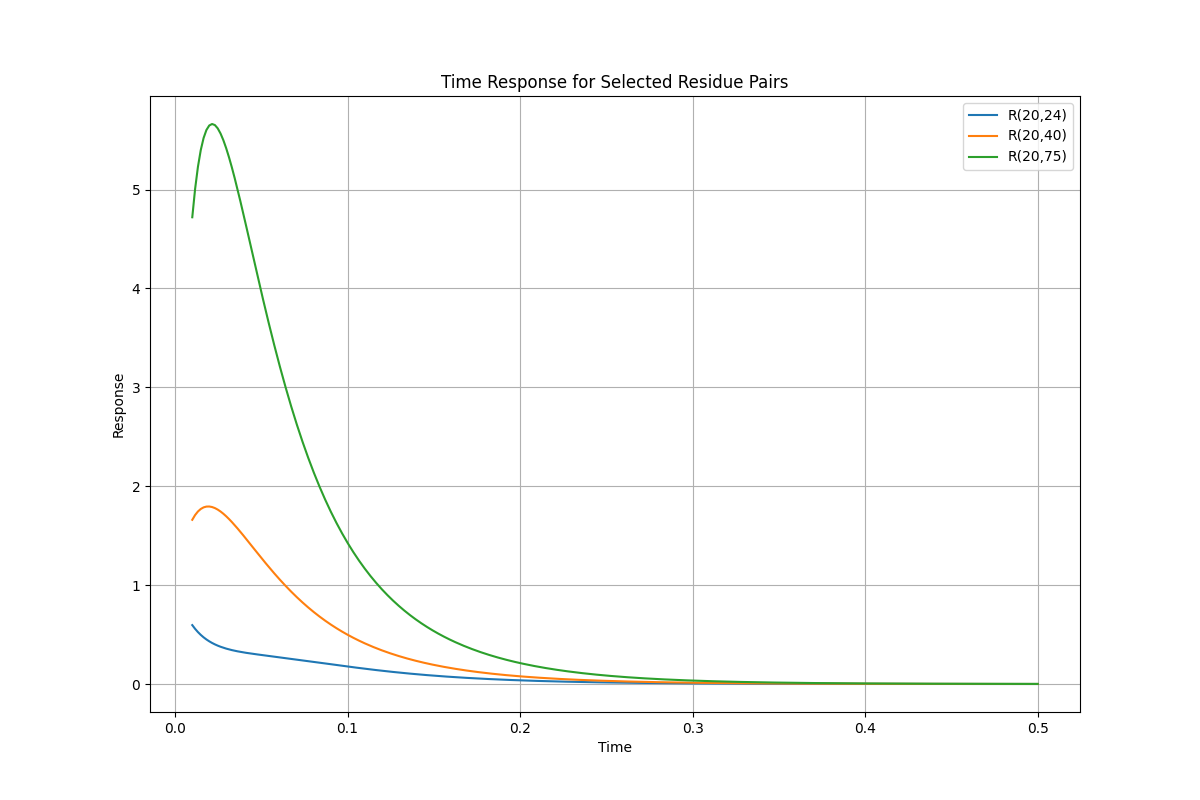
\includegraphics[width=0.5\textwidth]{"images/2m10Multiple_time_resposne.png"}
    \caption{Multiple time response}
\end{figure}

\begin{figure}[H]
    \centering
    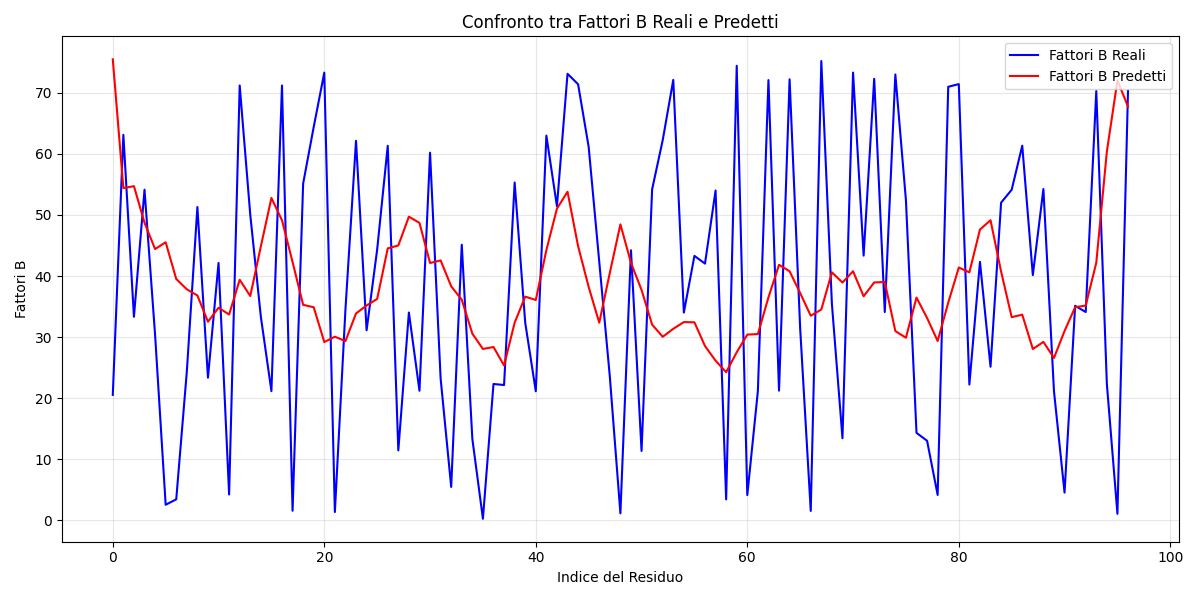
\includegraphics[width=0.5\textwidth]{"images/2m10Confronto tra Fattori B Reali e Predetti.png"}
    \caption{B factors}
\end{figure}
\begin{figure}[H]
    \centering
    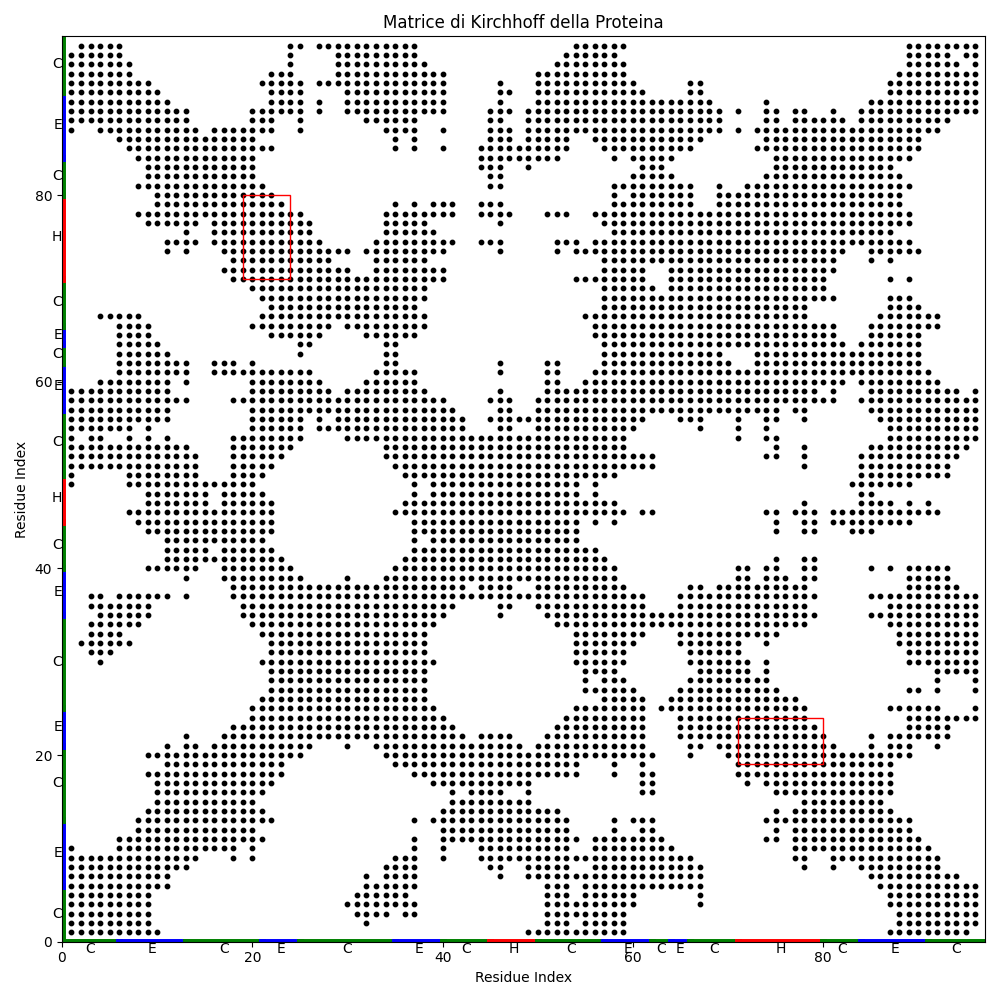
\includegraphics[width=0.5\textwidth]{"images/2m10_Matrice di Kirchhoff della Proteina.png"}
    \caption{Kirchhoff}
\end{figure}
\begin{figure}[H]
    \centering
    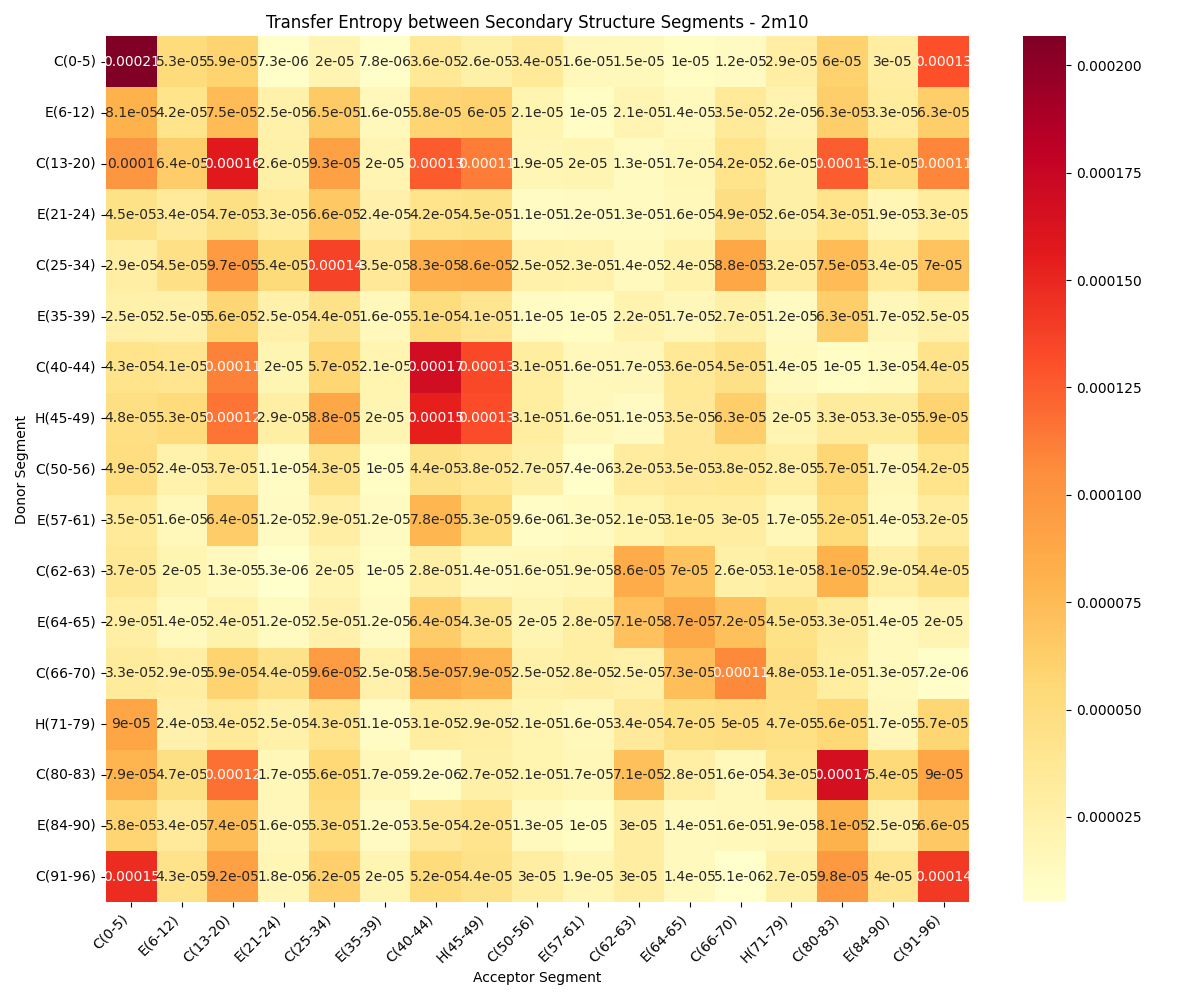
\includegraphics[width=0.5\textwidth]{"images/2m10analyze_secondary_structure_transfer_entropy.png"}
    \caption{Transfer struttura Secondaria}
\end{figure}
\section{3LNX}
\begin{figure}[H]
    \centering
    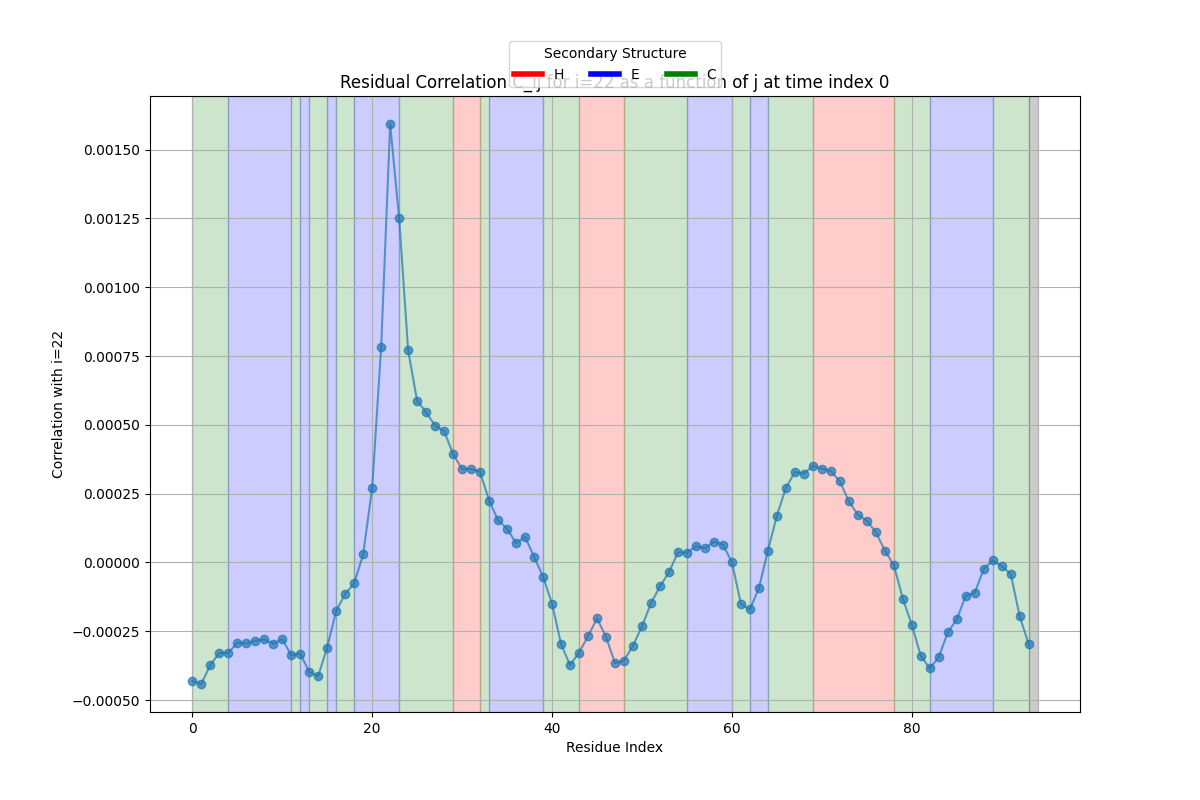
\includegraphics[width=0.5\textwidth]{"images/3LNXResidual Correlation C_ij for i=22 as a function of j at time index 0.png"}
    \caption{Correlazione}
\end{figure}
\begin{figure}[H]
    \centering
    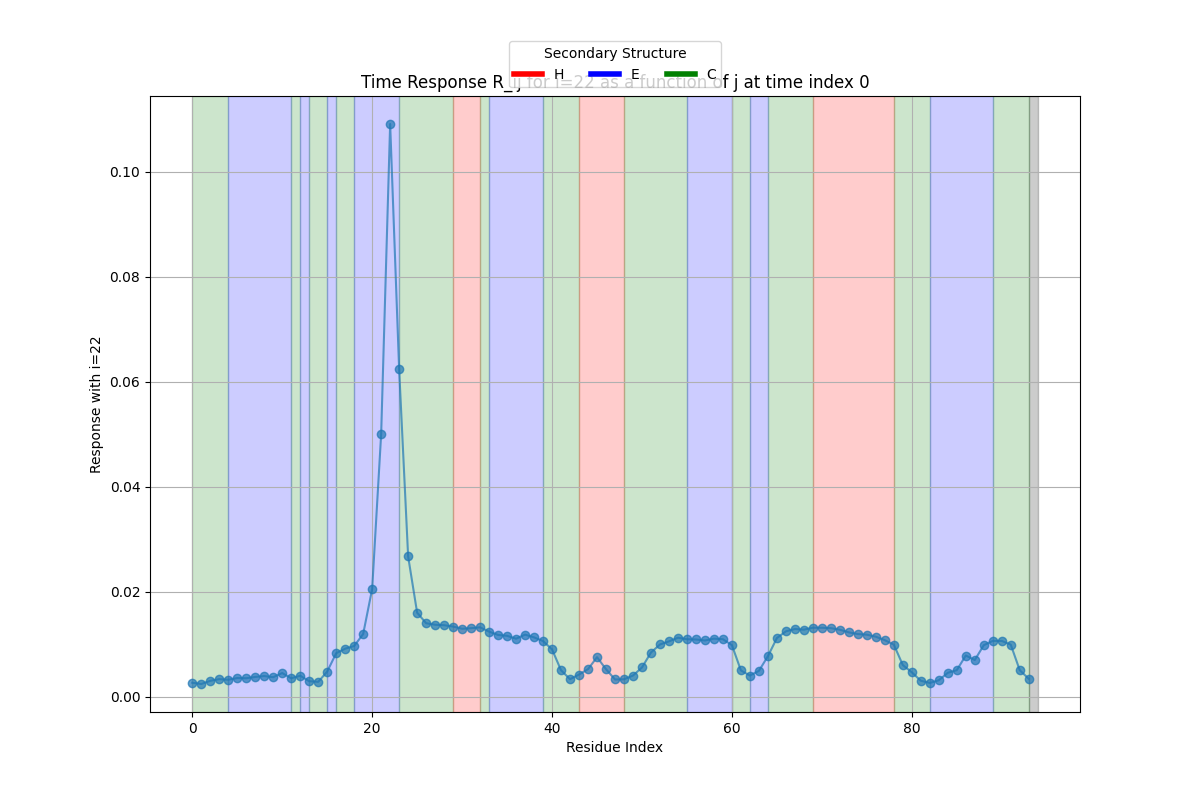
\includegraphics[width=0.5\textwidth]{"images/3LNXTime Response R_ij for i=22 as a function of j at time index 0.png"}
    \caption{Risposta}
\end{figure}

\begin{figure}[H]
    \centering
    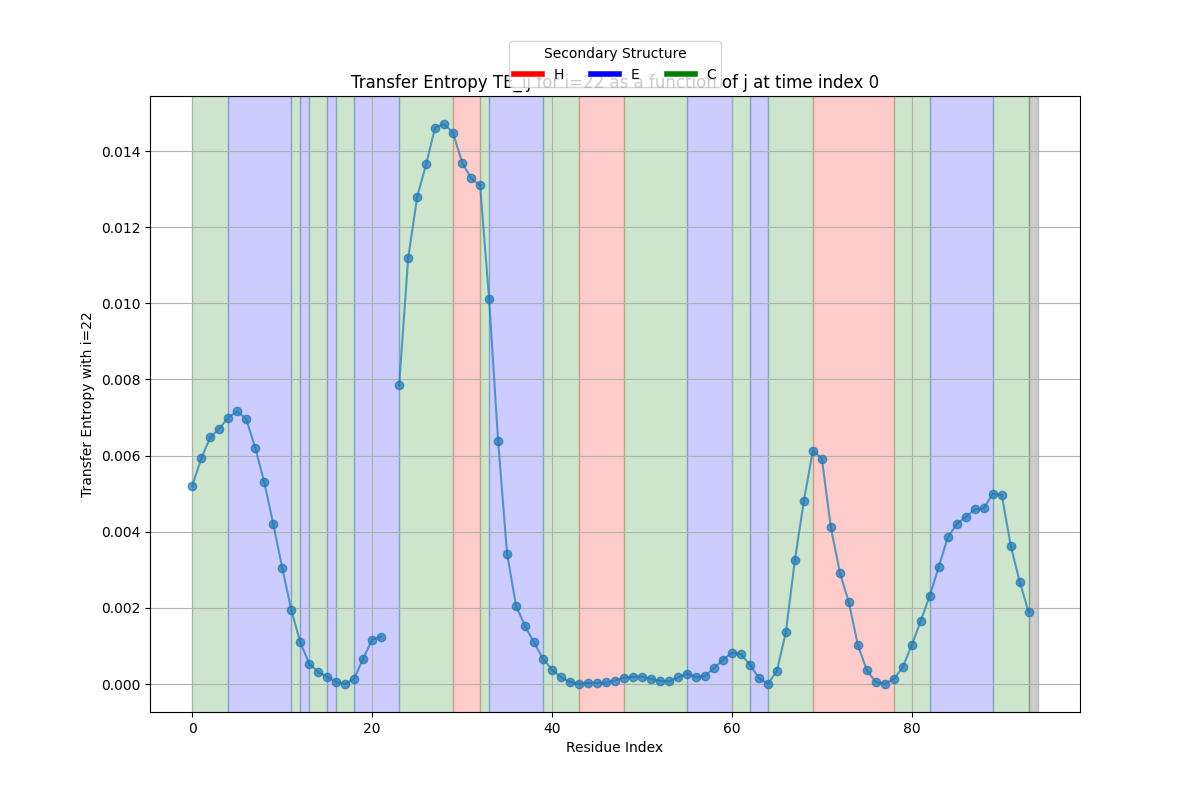
\includegraphics[width=0.5\textwidth]{"images/3LNXTransfer Entropy TE_ij for i=22 as a function of j at time index 0.png"}
    \caption{Transfer Entropy}
\end{figure}
\begin{figure}[H]
    \centering
    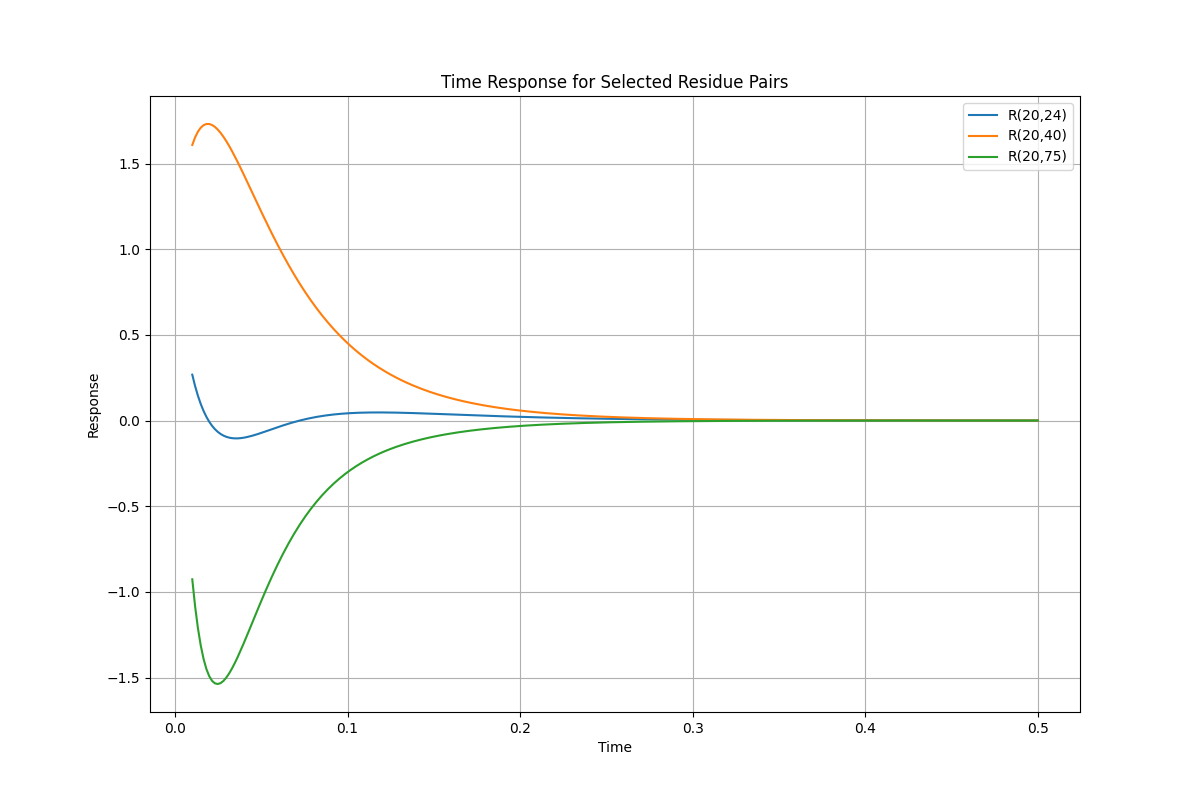
\includegraphics[width=0.5\textwidth]{"images/3LNXMultiple_time_resposne.png"}
    \caption{Multiple time response}
\end{figure}

\begin{figure}[H]
    \centering
    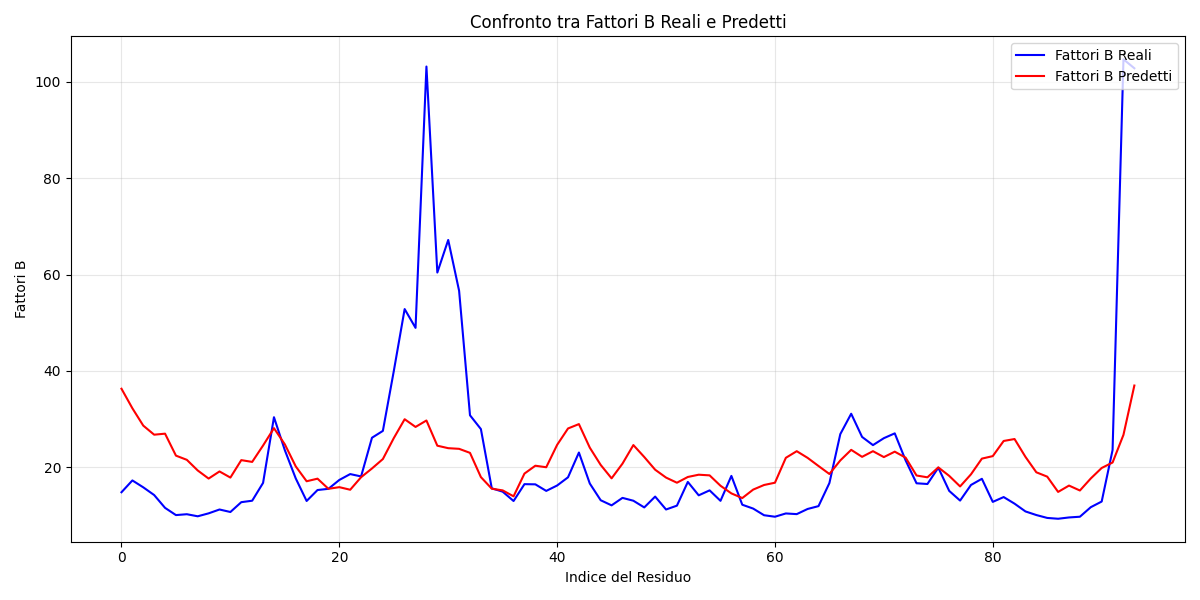
\includegraphics[width=0.5\textwidth]{"images/3LNXConfronto tra Fattori B Reali e Predetti.png"}
    \caption{B factors}
\end{figure}
\begin{figure}[H]
    \centering
    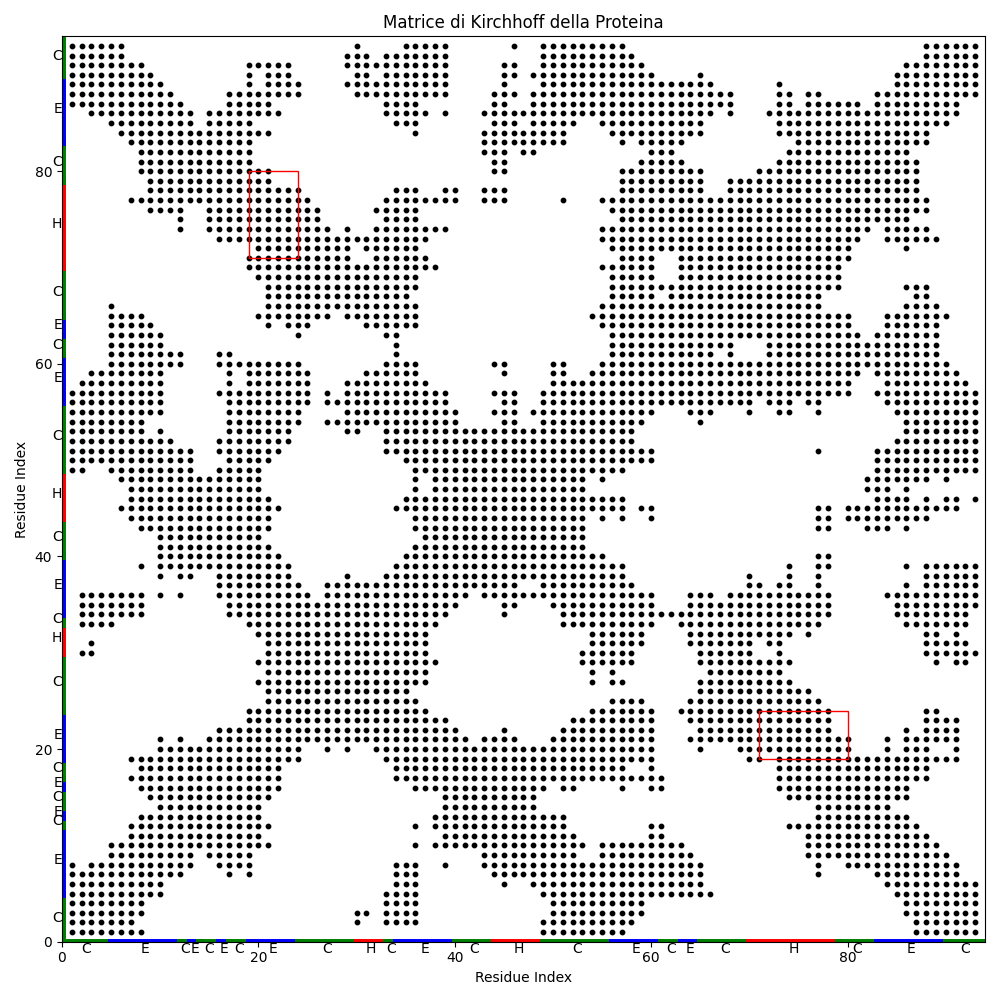
\includegraphics[width=0.5\textwidth]{"images/3LNX_Matrice di Kirchhoff della Proteina.png"}
    \caption{Kirchhoff}
\end{figure}
\begin{figure}[H]
    \centering
    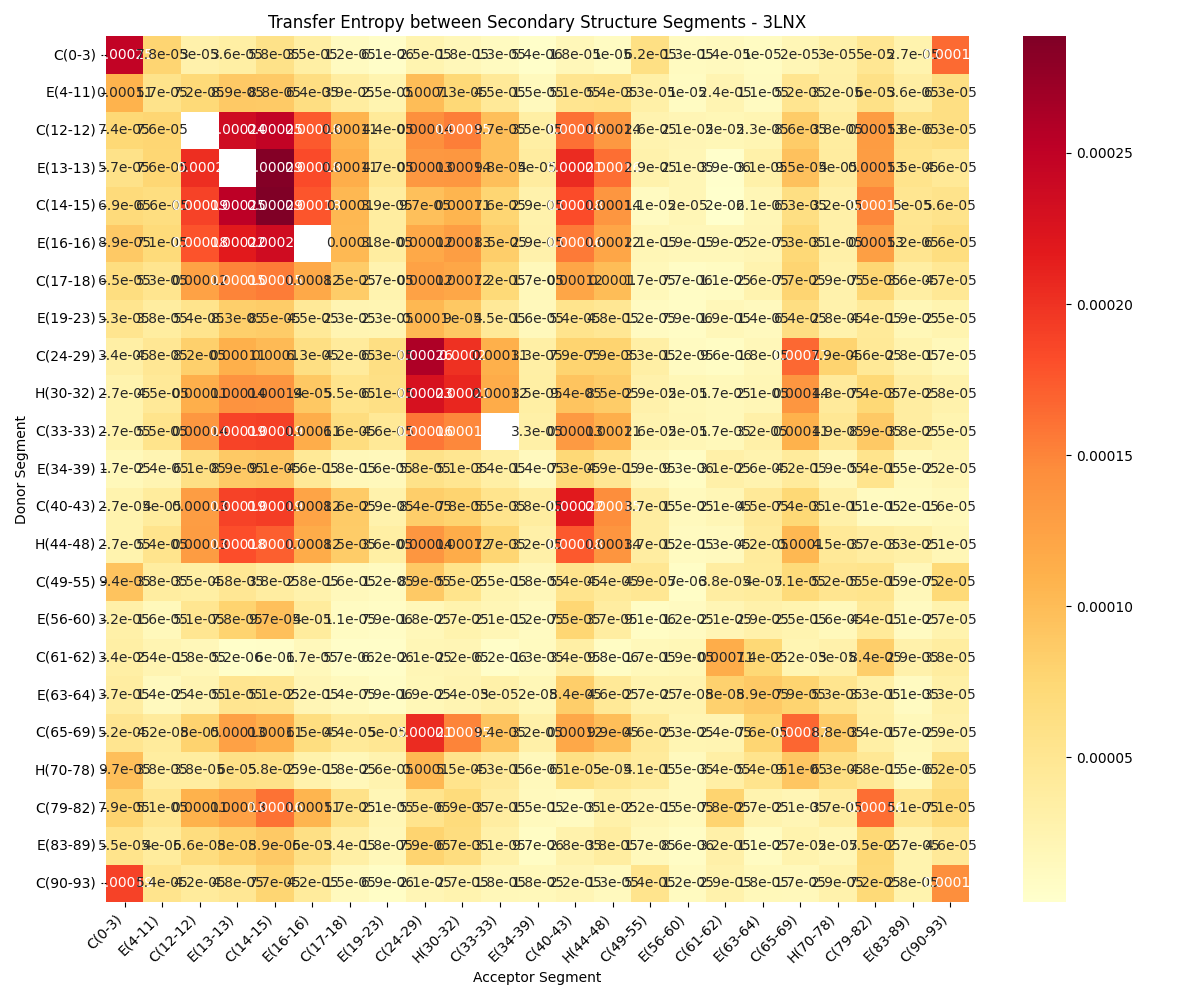
\includegraphics[width=0.5\textwidth]{"images/3LNXanalyze_secondary_structure_transfer_entropy.png"}
    \caption{Secondaria}
\end{figure}
\section{3LNY}
\begin{figure}[H]
    \centering
    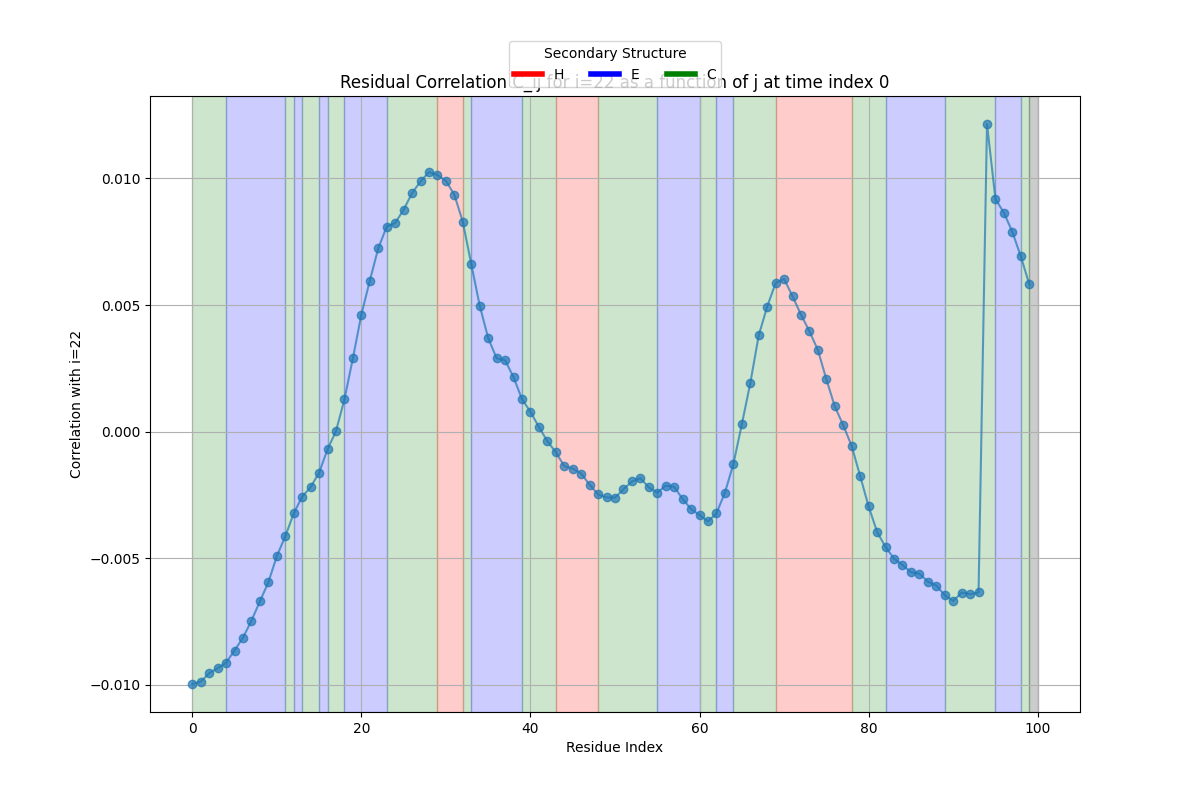
\includegraphics[width=0.5\textwidth]{"images/3LNYResidual Correlation C_ij for i=22 as a function of j at time index 0.png"}
    \caption{Correlazione}
\end{figure}
\begin{figure}[H]
    \centering
    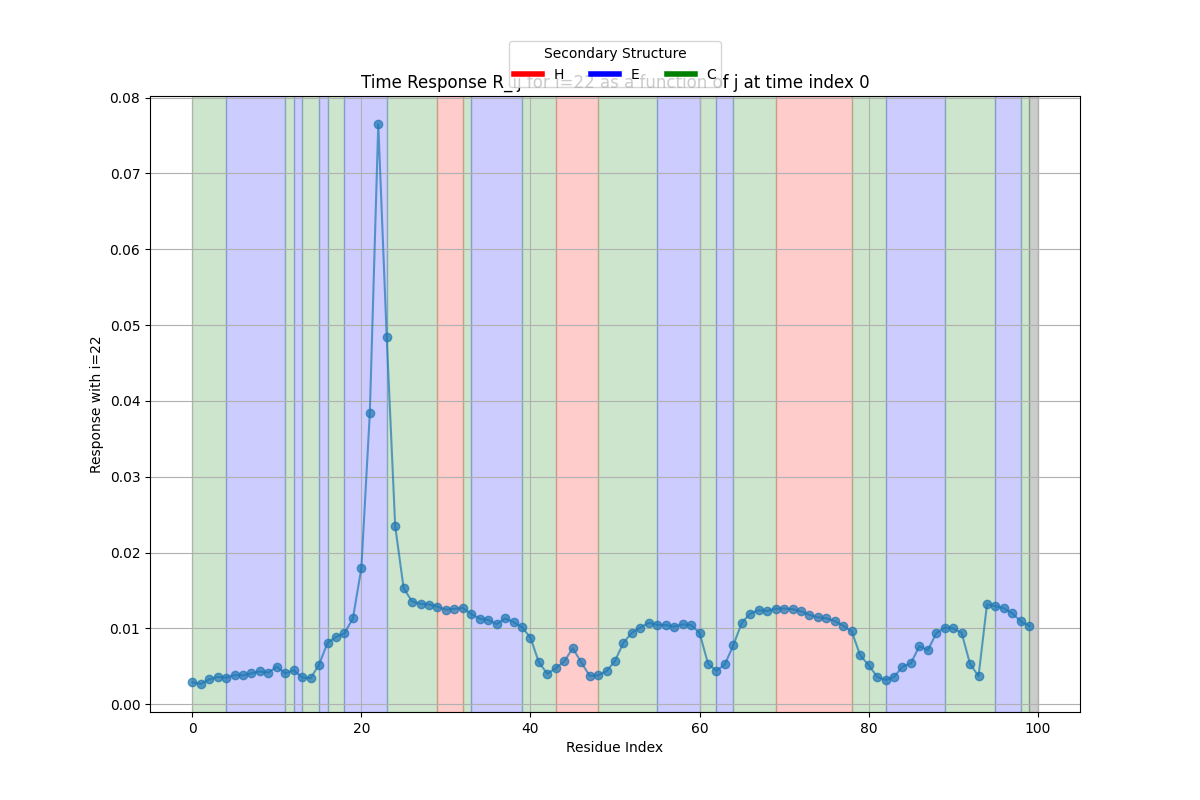
\includegraphics[width=0.5\textwidth]{"images/3LNYTime Response R_ij for i=22 as a function of j at time index 0.png"}
    \caption{Risposta}
\end{figure}

\begin{figure}[H]
    \centering
    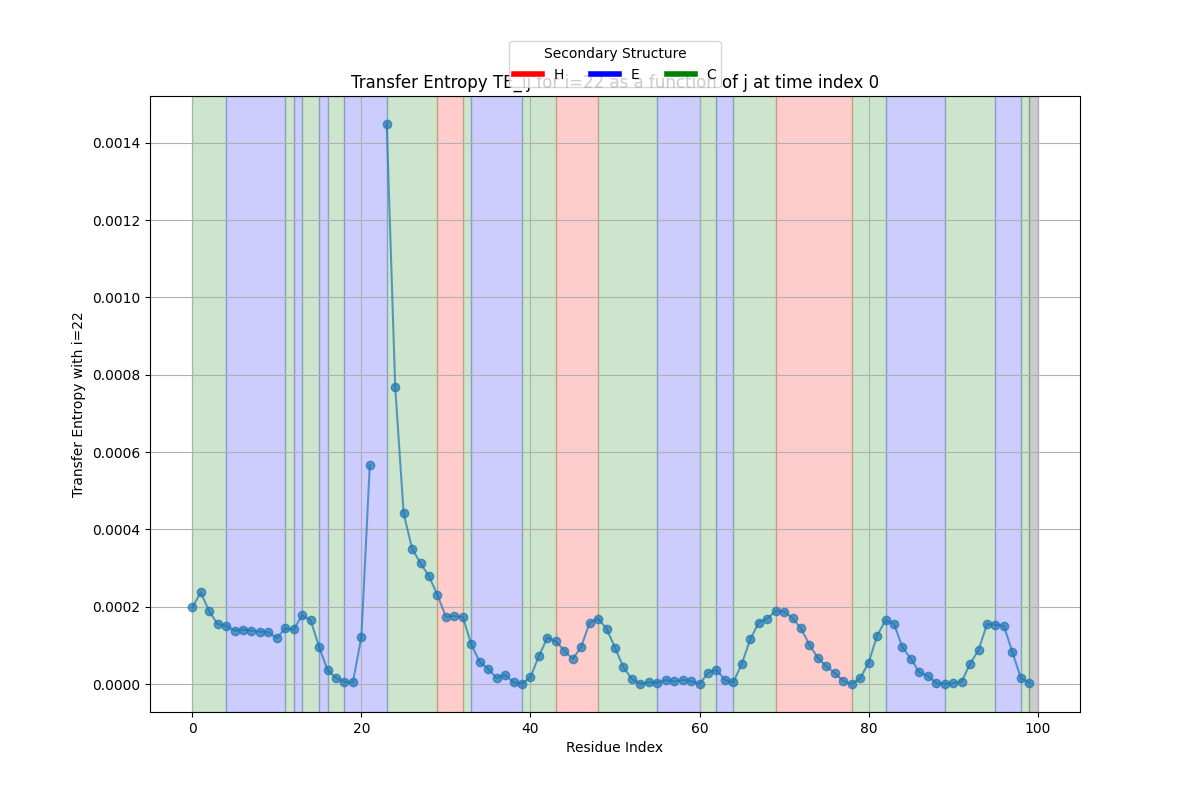
\includegraphics[width=0.5\textwidth]{"images/3LNYTransfer Entropy TE_ij for i=22 as a function of j at time index 0.png"}
    \caption{Transfer Entropy}
\end{figure}


\begin{figure}[H]
    \centering
    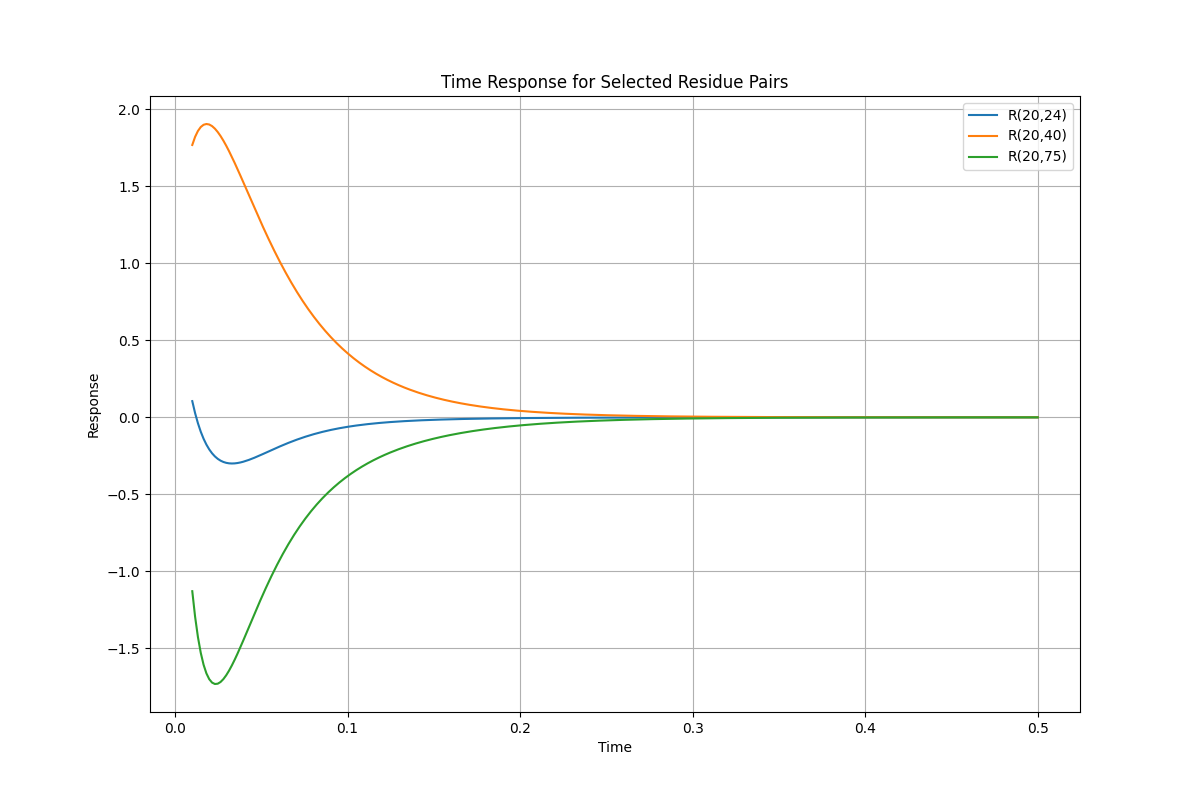
\includegraphics[width=0.5\textwidth]{"images/3LNYMultiple_time_resposne.png"}
    \caption{Multiple time response}
\end{figure}

\begin{figure}[H]
    \centering
    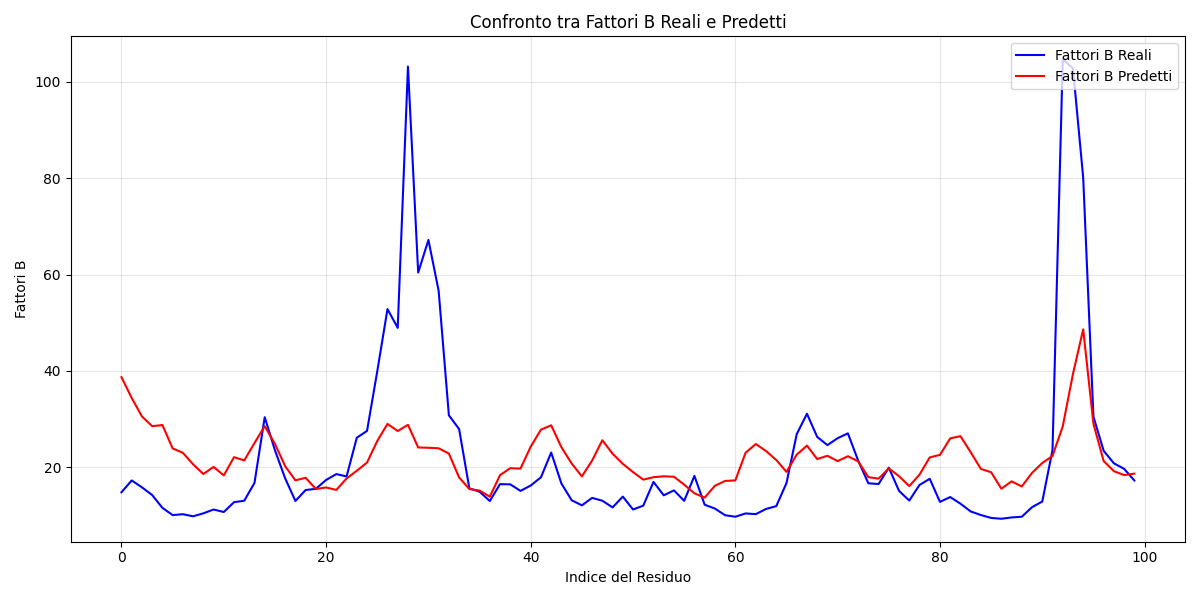
\includegraphics[width=0.5\textwidth]{"images/3LNYConfronto tra Fattori B Reali e Predetti.png"}
    \caption{B factors}
\end{figure}
\begin{figure}[H]
    \centering
    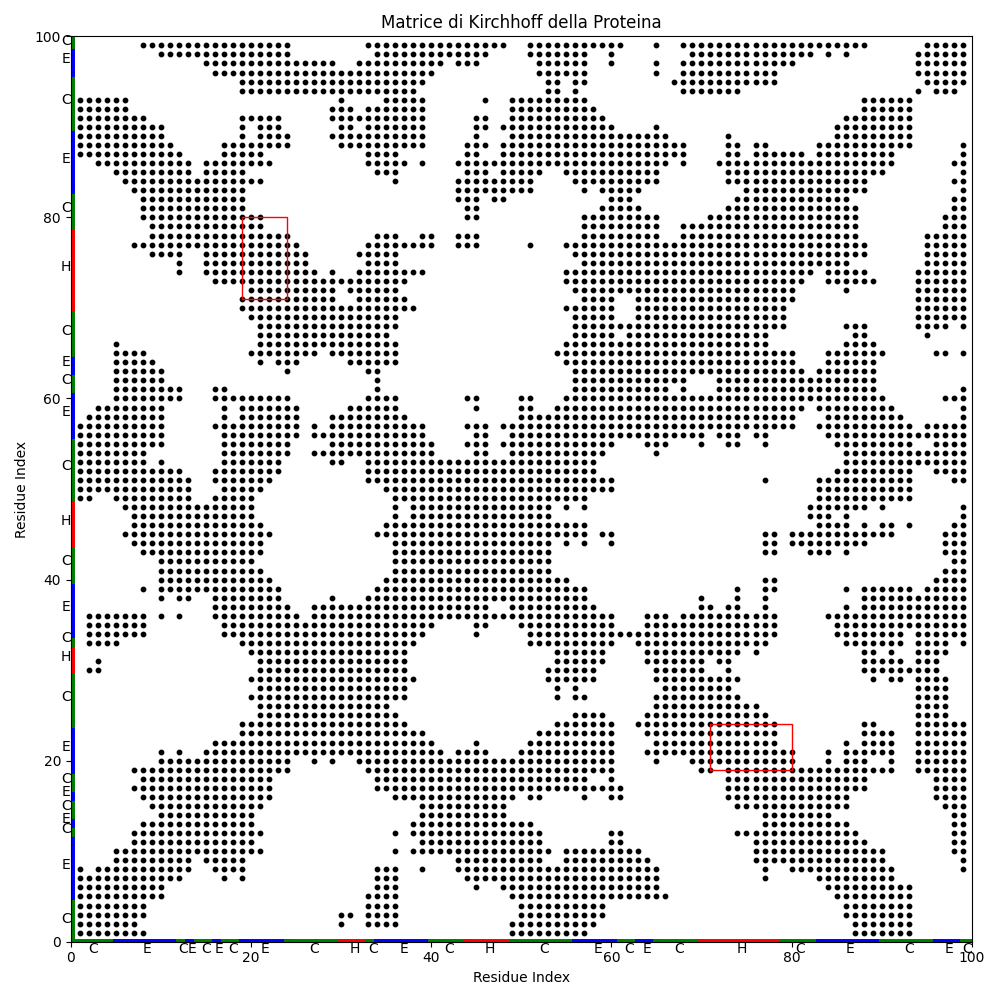
\includegraphics[width=0.5\textwidth]{"images/3LNY_Matrice di Kirchhoff della Proteina.png"}
    \caption{Kirchhoff}
\end{figure}
\begin{figure}[H]
    \centering
    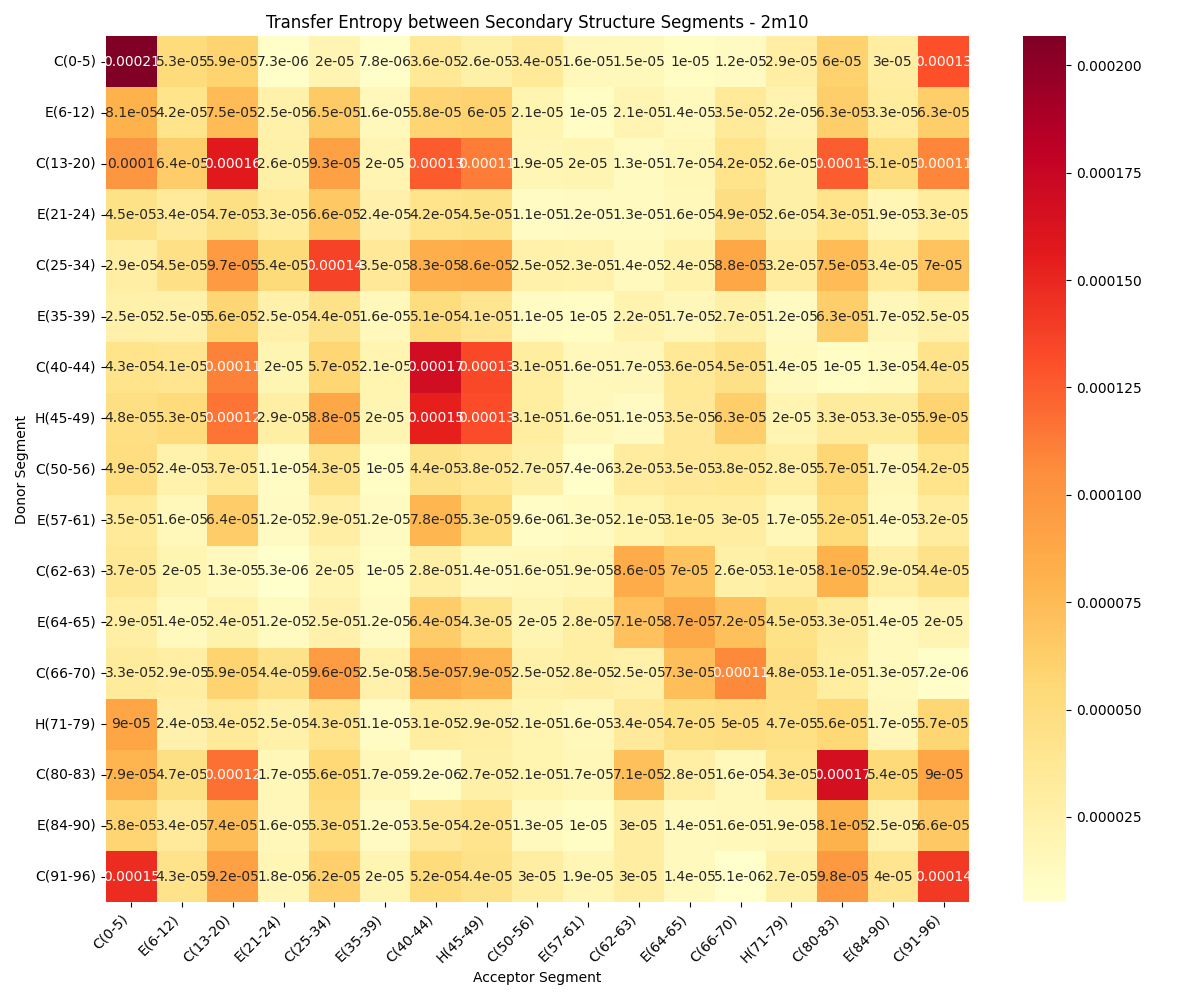
\includegraphics[width=0.5\textwidth]{"images/2m10analyze_secondary_structure_transfer_entropy.png"}
    \caption{Seocndaria}
\end{figure}
\section{Dinamica}
\begin{equation}
    \gamma \dot{x}_i = -g \sum_j K_{ij} x_j + \epsilon(t) (r_{21} - r_{76}) \delta_{i,21} - \epsilon(t) (r_{21} - r_{76}) \delta_{i,76} + \sqrt{2 \gamma k_B T} \xi_i(t)
    \end{equation}
Ora posso simulare il moto Time dependent di ogni atomo e vedere come si propagano le vibrazioni.
Gli autovalori sono smere le frequeze naturali del sistema.
\begin{figure}[H]
    \centering
    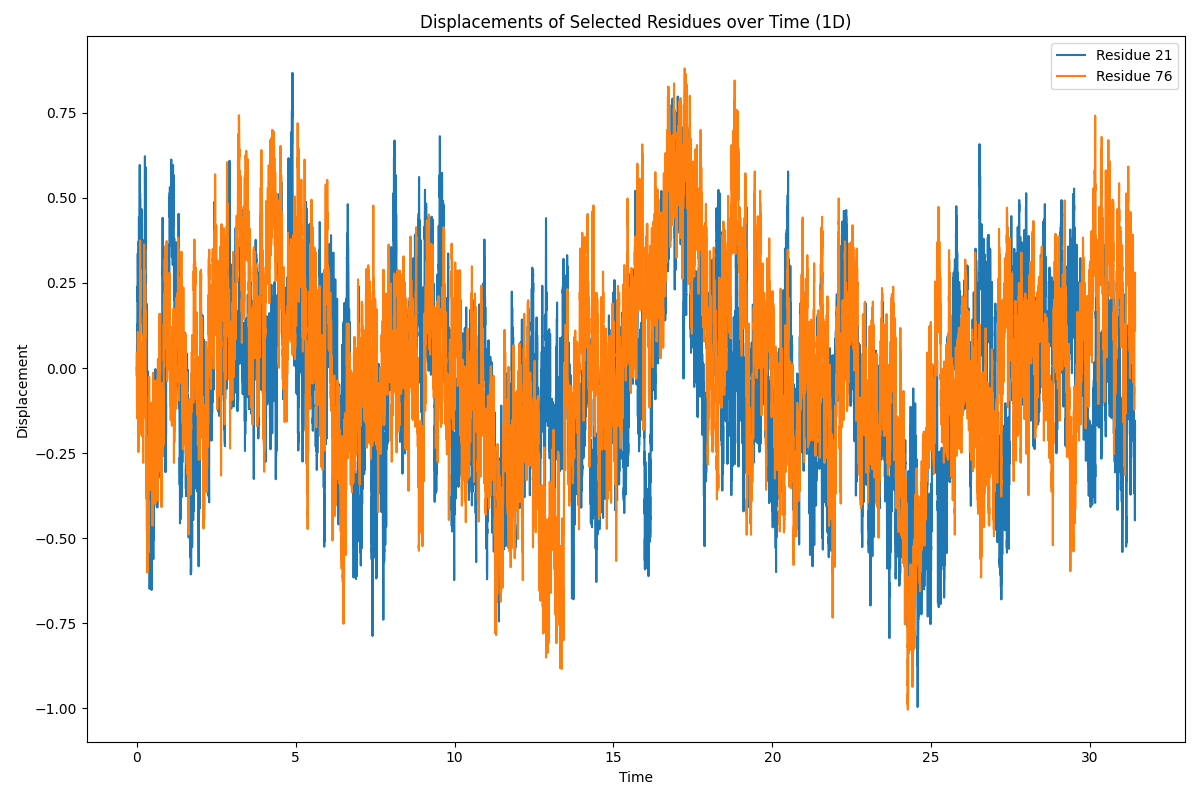
\includegraphics[width=0.5\textwidth]{"images/2m10_Processo_stocastico.png"}
    \caption{Seocndaria}
\end{figure}
\begin{figure}[H]
    \centering
    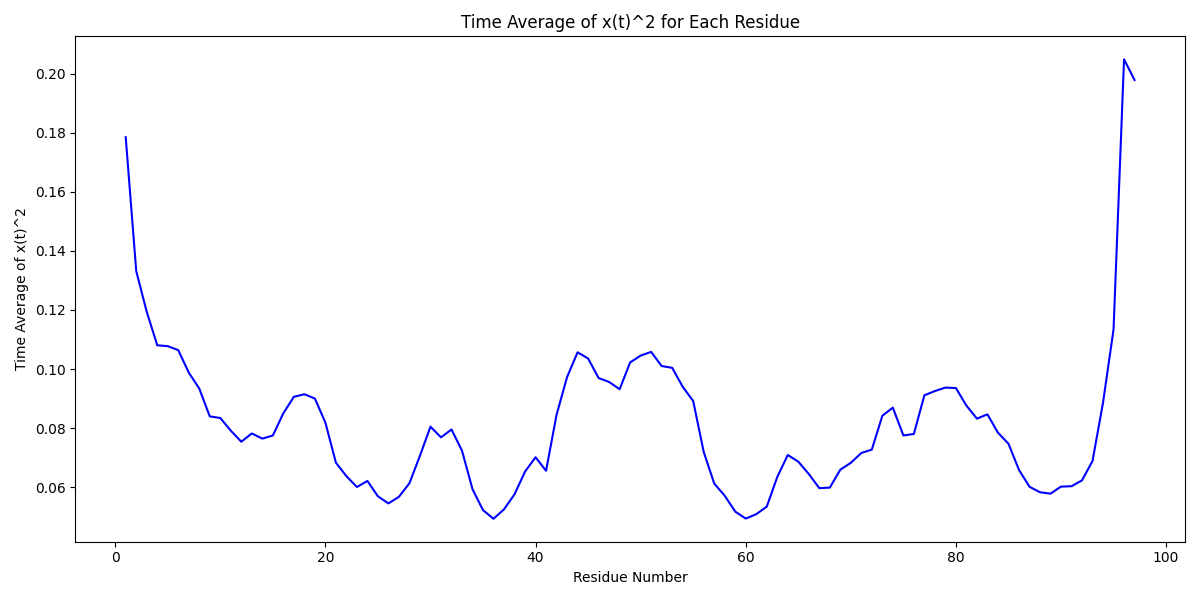
\includegraphics[width=0.5\textwidth]{"images/2m10_Stima beta factors.png"}
    \caption{Seocndaria}
\end{figure}
\section{Gradienete di temperature}
\begin{equation}
    \boldsymbol{\gamma}_i \dot{x}_i = -g \sum_j K_{ij} x_j  + \sqrt{2 \boldsymbol{\gamma}_i k_B \boldsymbol{T}_i} \xi_i(t)
    \end{equation}
Gamma e T sono diventati vettori.
Se la risolvi ottieni:
\begin{equation}
    \sum_{u} \exp\left( \sum_j K_{ij} u_j \right) \cdot \beta \cdot \beta^{\top} \cdot \exp\left( \sum_s K_{is} u_s \right)
    \end{equation}
Ora hai diversi modi di scegliere i valori di T:
\section{Troncamento Tmeperatura}
se sono sotto 5 legami allora ho temperatura bassa.
Se sono sopra allora ho temperatura piu' alta.
Posso prendere banalmente 2 valori 0,1 .
\begin{figure}[H]
    \centering
    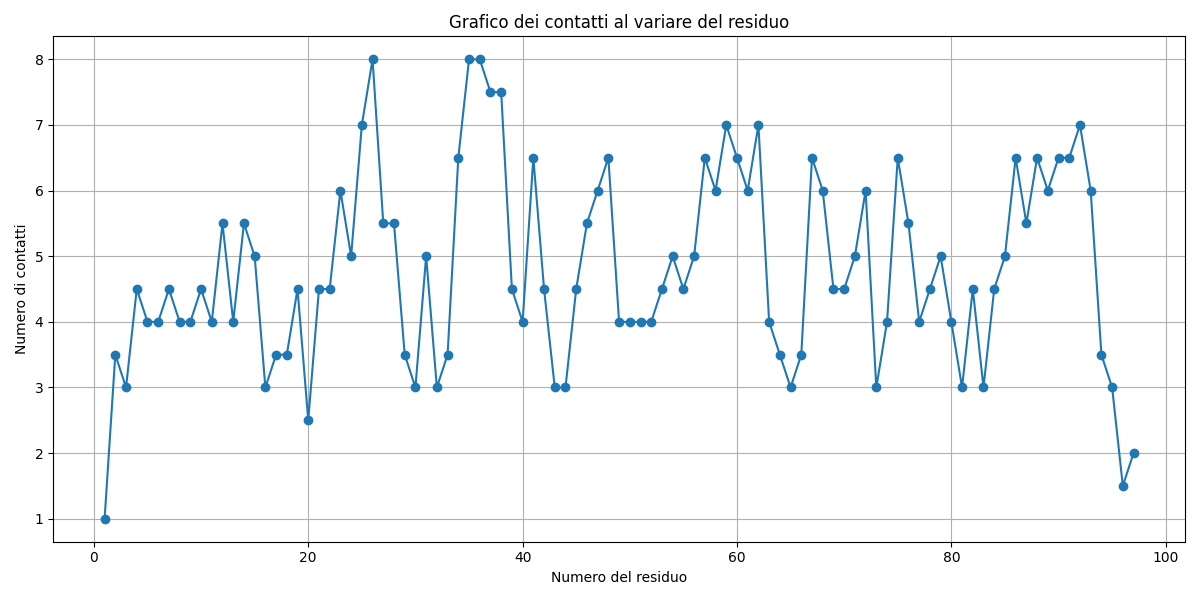
\includegraphics[width=0.5\textwidth]{"images/2m10_2_temperature_contact_cutoff.png"}
    \caption{ Temperatura Troncamento }
\end{figure}
\begin{figure}[H]
    \centering
    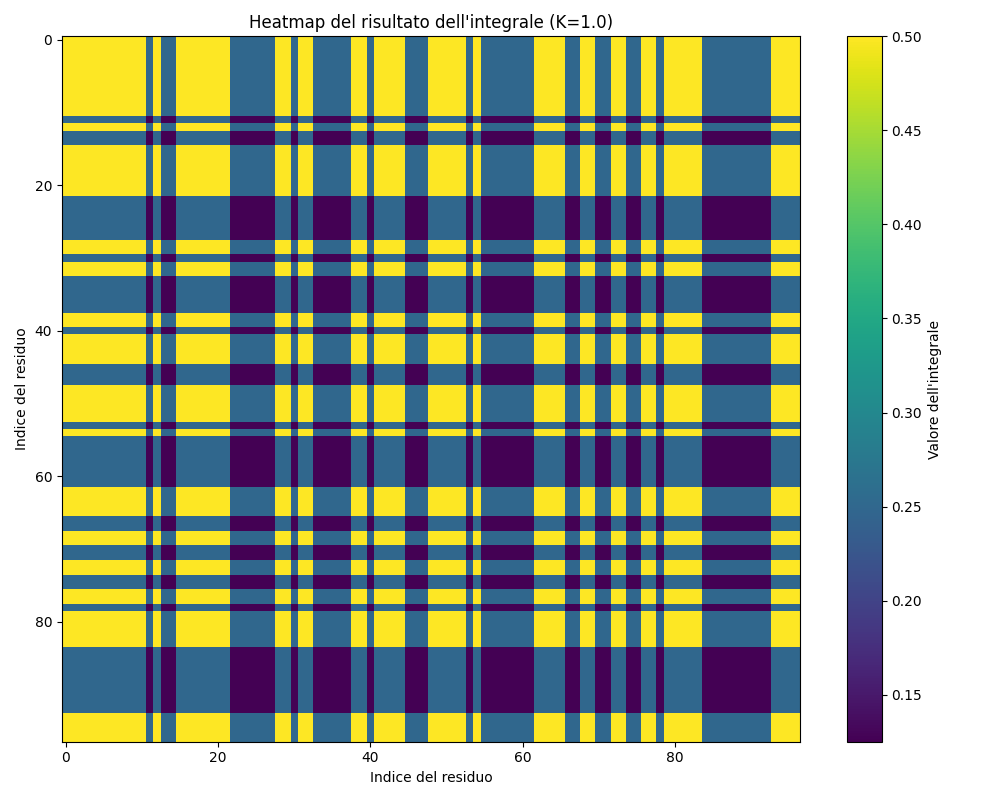
\includegraphics[width=0.5\textwidth]{"images/2m10_2_temperature_correlation_cutoff.png"}
    \caption{ Temperatura Troncamento  }
\end{figure}
\begin{figure}[H]
    \centering
    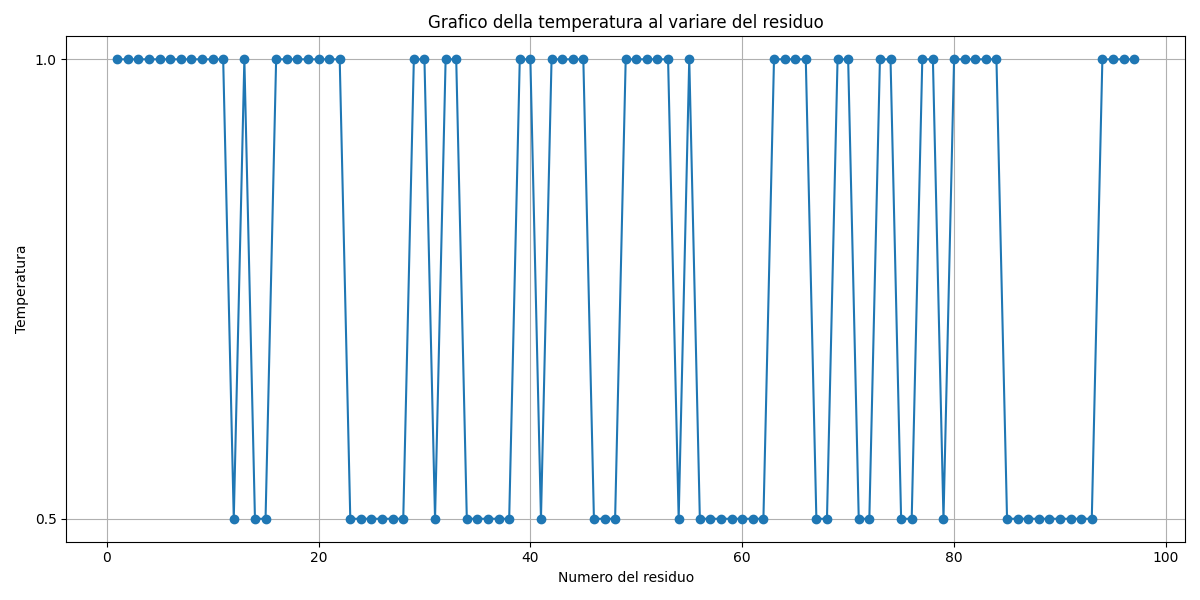
\includegraphics[width=0.5\textwidth]{"images/2m10_2_temperature_cutoff.png"}
    \caption{ Temperatura Troncamento  }
\end{figure}

\section{Temperatura radiale}
T(r)=T_0+(Tb-T0)/R*r

\begin{figure}[H]
    \centering
    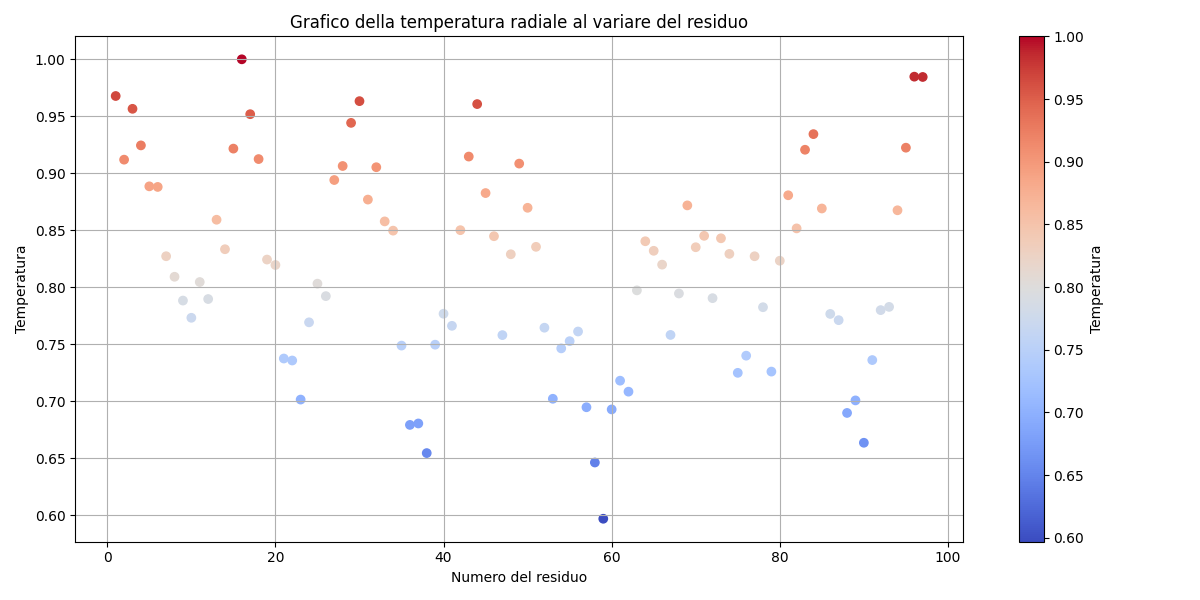
\includegraphics[width=0.5\textwidth]{"images/2m10_2_temperature_sferic.png"}
    \caption{Temperatura Radiale}
\end{figure}
\begin{figure}[H]
    \centering
    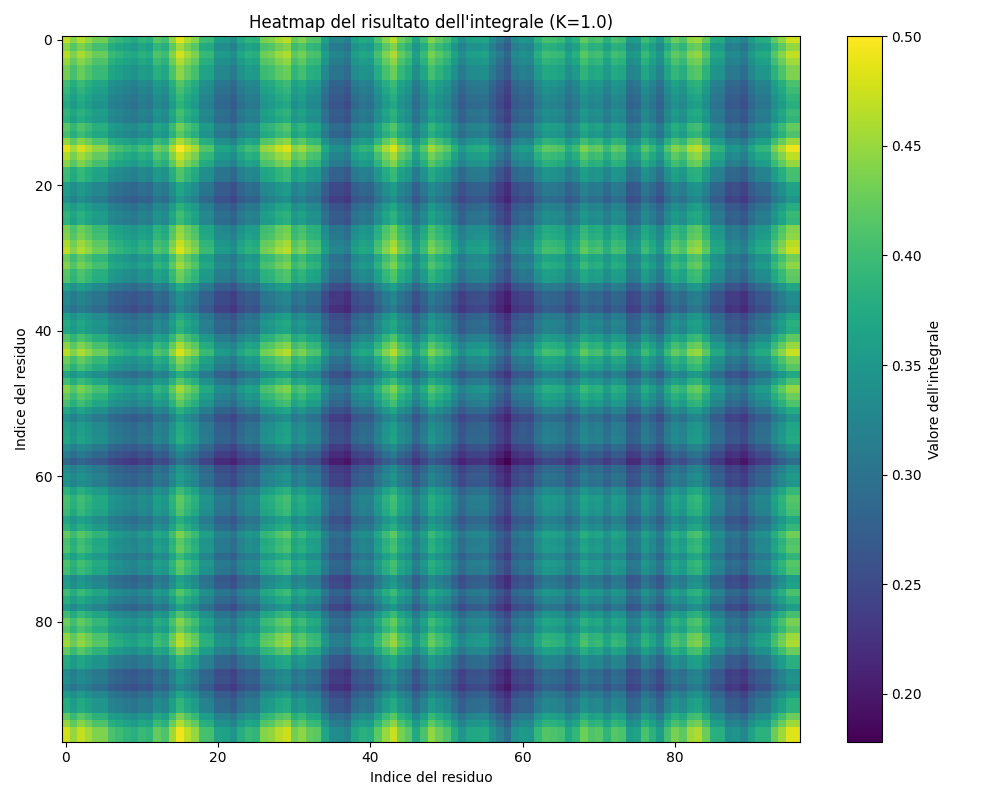
\includegraphics[width=0.5\textwidth]{"images/2m10_2_temperature_correlation_sferic.png"}
    \caption{Correlazione Radiale}
\end{figure}






\section*{Risoluzione dell'equazione differenziale e calcolo della correlazione}

Partiamo dall'equazione differenziale data per \( x_i(t) \):

\[
\frac{dx_i}{dt} = -\sum_j K_{ij} x_j + \sqrt{2 k_B T} \, \eta_i + \left(1 - \cos(\omega t)\right)(\delta_{a_i} - \delta_{b_i})
\]

dove:
- \( K_{ij} \) rappresenta la matrice di accoppiamento tra i nodi,
- \( \eta_i \) è un processo di Wiener (rumore bianco gaussiano) con \(\langle \eta_i(t) \eta_j(s) \rangle = \delta_{ij} \delta(t - s)\),
- \( \delta_{a_i} \) e \( \delta_{b_i} \) sono costanti di offset che definiscono la parte oscillatoria del sistema.

### Passaggio agli autovettori

Definiamo il cambiamento di base usando gli autovettori della matrice \( K \), scrivendo:

\[
x_i(t) = \sum_k V_{ik} Q_k(t)
\]

dove \( V \) è la matrice degli autovettori di \( K \), e \( Q_k(t) \) rappresenta la dinamica lungo ciascun autovettore. L'equazione differenziale per \( Q_k(t) \) diventa:

\[
\frac{dQ_k}{dt} = -\lambda_k Q_k + C_k (1 - \cos(\omega t)) + \sqrt{2 k_B T} \, \tilde{\eta}_k
\]

con:
- \( \lambda_k \) autovalori associati agli autovettori di \( K \),
- \( C_k = \sum_i V_{ik} (\delta_{a_i} - \delta_{b_i}) \),
- \( \tilde{\eta}_k = \sum_i V_{ik} \eta_i \) è il rumore proiettato sugli autovettori.

### Soluzione dell'equazione differenziale per \( Q_k(t) \)

La soluzione formale per \( Q_k(t) \) è data dalla somma di una parte deterministica e di una parte stocastica:

\[
Q_k(t) = Q_k^{\text{det}}(t) + Q_k^{\text{rumore}}(t)
\]

1. **Parte deterministica**: Integrando la parte deterministica, otteniamo

   \[
   Q_k^{\text{det}}(t) = C_k \left( \frac{1 - e^{-\lambda_k t}}{\lambda_k} - \frac{e^{-\lambda_k t} - \cos(\omega t) + \frac{\lambda_k}{\omega} \sin(\omega t)}{\lambda_k^2 + \omega^2} \right)
   \]

2. **Parte stocastica**: La soluzione per la parte stocastica dovuta al rumore è

   \[
   Q_k^{\text{rumore}}(t) = \sqrt{2 k_B T} \int_0^t e^{-\lambda_k (t - u)} \tilde{\eta}_k(u) \, du
   \]

   ### Calcolo della correlazione \(\langle x_i(t) x_j(s) \rangle\)

   La correlazione media \(\langle x_i(t) x_j(s) \rangle\) è:
   
   \[
   \langle x_i(t) x_j(s) \rangle = \sum_{k, l} V_{ik} V_{jl} \langle Q_k(t) Q_l(s) \rangle,
   \]
   
   dove \(\langle Q_k(t) Q_l(s) \rangle\) può essere suddivisa nei contributi deterministico e stocastico:
   
   \[
   \langle Q_k(t) Q_l(s) \rangle = \langle Q_k^{\text{det}}(t) Q_l^{\text{det}}(s) \rangle + \langle Q_k^{\text{rumore}}(t) Q_l^{\text{rumore}}(s) \rangle.
   \]
   
   #### Contributo deterministico
   
   La correlazione tra le parti deterministiche è:
   
   \[
   \langle Q_k^{\text{det}}(t) Q_k^{\text{det}}(s) \rangle = C_k^2 \left( f_k(t, s) + g_k(t, s) \cos(\omega (t - s)) + h_k(t, s) \sin(\omega (t - s)) \right),
   \]
   
   dove:
   - \( f_k(t, s) \) rappresenta il termine di decadimento esponenziale dato da:
     \[
     f_k(t, s) = \frac{(1 - e^{-\lambda_k t})(1 - e^{-\lambda_k s})}{\lambda_k^2},
     \]
   - \( g_k(t, s) \) rappresenta il termine di correlazione coseno:
     \[
     g_k(t, s) = \frac{e^{-\lambda_k(t+s)} - \cos(\omega t) \cos(\omega s)}{\lambda_k^2 + \omega^2},
     \]
   - \( h_k(t, s) \) rappresenta il termine di correlazione seno:
     \[
     h_k(t, s) = \frac{\lambda_k (\sin(\omega t) \cos(\omega s) + \cos(\omega t) \sin(\omega s))}{\lambda_k^2 + \omega^2}.
     \]
   
   #### Contributo stocastico
   
   Per la parte stocastica, otteniamo:
   
   \[
   \langle Q_k^{\text{rumore}}(t) Q_k^{\text{rumore}}(s) \rangle = \frac{k_B T}{\lambda_k} \delta_{kl} e^{-\lambda_k |t - s|}.
   \]
   
   ### Risultato finale
   
   Combinando i termini, otteniamo la correlazione media finale per \(\langle x_i(t) x_j(s) \rangle\):
   
   \[
   \langle x_i(t) x_j(s) \rangle = \sum_k V_{ik} V_{jk} \left( C_k^2 \left( f_k(t, s) + g_k(t, s) \cos(\omega (t - s)) + h_k(t, s) \sin(\omega (t - s)) \right) + \frac{k_B T}{\lambda_k} e^{-\lambda_k |t - s|} \right).
   \]
   
   Ogni termine è ora chiaramente identificato:
   - \( C_k^2 f_k(t, s) \): componente di decadimento esponenziale,
   - \( C_k^2 g_k(t, s) \cos(\omega (t - s)) \): componente oscillatoria con coseno,
   - \( C_k^2 h_k(t, s) \sin(\omega (t - s)) \): componente oscillatoria con seno,
   - \( \frac{k_B T}{\lambda_k} e^{-\lambda_k |t - s|} \): contributo del rumore termico.
   

   
   

\section*{Produzione di Entropia}

La produzione di entropia \( S \) può essere calcolata utilizzando l'espressione data per la forza \( F \) e l'equazione differenziale associata al sistema.

\subsection*{Equazione Differenziale}

Consideriamo l'equazione differenziale:

\[
\frac{dx_i}{dt} = -\sum_j K_{ij} x_j + \sqrt{2 k_B T} \eta_i + (1 - \cos(\omega t)) (\delta_{a_i} - \delta_{b_i}).
\]

\subsection*{Espressione per \( F \)}

L'espressione per \( F \) è data da:

\[
F = \sum_j K_{ij} x_j + (1 - \cos(\omega t)) (\delta_{a_i} - \delta_{b_i}).
\]

\subsection*{Produzione di Entropia}

La produzione di entropia può essere espressa come:

\[
S = \frac{F \cdot \frac{dx}{dt}}{T}.
\]

Sostituendo \( F \) e \( \frac{dx}{dt} \), otteniamo:

1. Sostituendo \( F \):

\[
F = \sum_j K_{ij} x_j + (1 - \cos(\omega t)) (\delta_{a_i} - \delta_{b_i}).
\]

2. Sostituendo \( \frac{dx}{dt} \):

\[
\frac{dx_i}{dt} = -\sum_k K_{ik} x_k + \sqrt{2 k_B T} \eta_i + (1 - \cos(\omega t)) (\delta_{a_i} - \delta_{b_i}).
\]

\subsection*{Produzione di Entropia Completa}

Pertanto, la produzione di entropia può essere scritta come:


\[
S = \frac{1}{T} \left[ \sum_j K_{ij} x_j \left( -\sum_k K_{ik} x_k + \sqrt{2 k_B T} \eta_i + (1 - \cos(\omega t)) (\delta_{a_i} - \delta_{b_i}) \right) + (1 - \cos(\omega t)) (\delta_{a_i} - \delta_{b_i}) \left( -\sum_k K_{ik} x_k + \sqrt{2 k_B T} \eta_i + (1 - \cos(\omega t)) (\delta_{a_i} - \delta_{b_i}) \right) \right].
\]


\subsection*{Considerazioni sulle Semplificazioni}

Esploriamo ora alcune possibili semplificazioni dell'espressione per la produzione di entropia:

\begin{enumerate}
    \item \textbf{Condizioni di Equilibrio}: Se il sistema è in equilibrio termico, potremmo avere \( \langle x_j \rangle \) costante, semplificando il calcolo della somma sui termini di \( K_{ij} x_j \).
    
    \item \textbf{Media Temporale}: Considerando la media temporale di \( S \), alcuni termini oscillatori (come quelli con \( \cos(\omega t) \)) potrebbero cancellarsi nel lungo termine, specialmente se le oscillazioni sono simmetriche attorno a zero.
    
    \item \textbf{Domini di Oscillazione}: Se i contributi oscillatori non sono dominanti, potremmo trascurarli per un'analisi qualitativa.
    
    \item \textbf{Assunzione di Piccole Oscillazioni}: Se le oscillazioni sono piccole, possiamo linearizzare i termini, ma questa assunzione potrebbe non essere sempre valida a seconda dell'ampiezza delle oscillazioni.
\end{enumerate}

\subsection*{Conclusioni}

In generale, mentre l'espressione per la produzione di entropia è complessa, alcune semplificazioni possono essere applicabili in condizioni specifiche, come stati di equilibrio o considerando medie temporali. Tuttavia, senza ulteriori informazioni sulle dinamiche del sistema o sul comportamento dei termini, non è facile ottenere una forma significativamente più semplice dell'espressione.




\section{Fokker planck N temperature}

L'equazione di Fokker-Planck associata all'equazione differenziale

\[
\frac{dx_i}{dt} = -\sum_j K_{ij} x_j + B \eta_i
\]

è data da:

\[
\frac{\partial P(x,t)}{\partial t} = \sum_i \frac{\partial}{\partial x_i} \left[ \sum_j K_{ij} x_j P \right] + \frac{1}{2} \sum_{i,j} \frac{\partial^2}{\partial x_i \partial x_j} \left[ B_{ii} \delta_{ij} P \right]
\]

dove:
\begin{itemize}
    \item \( P(x,t) \) è la densità di probabilità del sistema,
    \item \( A_i = -\sum_j K_{ij} x_j \) è il termine drift,
    \item \( D_{ij} = B_{ii} \delta_{ij} \) è la matrice di diffusione.
\end{itemize}





\section*{Soluzione dell'Equazione Differenziale}

Consideriamo l'equazione differenziale iniziale:

\[
\frac{\partial P}{\partial t} = \sum_i \left( \sum_j K_{ij} x_j P \right) + 0.5 \sum_{i,j} \left( \frac{\partial^2}{\partial x_i \partial x_j} (B_{ij} P) \right).
\]

Dove \( P = P(x, t) \), \( K \) è la matrice di Kirchhoff e \( B \) è una matrice diagonale.

Supponiamo una condizione iniziale:

\[
P(x, 0) = \delta(x - x_0).
\]

\subsection*{Trasformata di Fourier}

Applicando la trasformata di Fourier rispetto a \( x \):

\[
P(k, t) = \int_{-\infty}^{+\infty} P(x, t) e^{-ikx} \, dx.
\]

La trasformata dell'equazione diventa:

\[
\frac{\partial P(k, t)}{\partial t} = \int_{-\infty}^{+\infty} \left( \sum_i \left( \sum_j K_{ij} x_j P \right) \right) e^{-ikx} \, dx + 0.5 \int_{-\infty}^{+\infty} \left( \sum_{i,j} \frac{\partial^2}{\partial x_i \partial x_j} (B_{ij} P) \right) e^{-ikx} \, dx.
\]

\subsection*{Primo Termine: Derivata e Trasformata}

Focalizziamoci sul primo termine:

\[
\frac{\partial P(k, t)}{\partial t} = \sum_i \left( K_{ii} P(k, t) \right) + \sum_{i,j} K_{ij} \left( \int_{-\infty}^{+\infty} x_j P(x, t) e^{-ikx} \, dx \right).
\]

Per il secondo termine, utilizziamo la proprietà della trasformata di Fourier per la derivata:

\[
\int_{-\infty}^{+\infty} \frac{\partial^2 P}{\partial x_i \partial x_j} e^{-ikx} \, dx = -k_i k_j P(k, t).
\]

Quindi, l'equazione diventa:

\[
\frac{\partial P(k, t)}{\partial t} = \sum_i K_{ii} P(k, t) + \sum_{i,j} K_{ij} \left( -i \frac{\partial P(k, t)}{\partial k} \right) - 0.5 \sum_{i,j} B_{ij} k_i k_j P(k, t).
\]

\subsection*{Semplificazione}

Riorganizzando l'equazione, otteniamo:

\[
\frac{\partial P(k, t)}{\partial t} = \sum_i K_{ii} P(k, t) + \sum_{i,j} K_{ij} \left( -ik_j P(k, t) \right) - 0.5 \sum_{i,j} B_{ij} k_i k_j P(k, t).
\]

Definiamo \(\Lambda(k)\):

\[
\Lambda(k) = \sum_i K_{ii} + \sum_{i,j} K_{ij} (-ik_j) - 0.5 \sum_{i,j} B_{ij} k_i k_j.
\]

Quindi, l'equazione diventa:

\[
\frac{\partial P(k, t)}{\partial t} = \Lambda(k) P(k, t).
\]

\subsection*{Risoluzione dell'Equazione Differenziale}

La soluzione dell'equazione differenziale è:

\[
P(k, t) = P(k, 0) e^{\Lambda(k) t}.
\]

Utilizzando la condizione iniziale \( P(k, 0) = e^{-ikx_0} \):

\[
P(k, t) = e^{-ikx_0} e^{\Lambda(k) t}.
\]

\subsection*{Trasformata Inversa}

Per trovare \( P(x, t) \), applichiamo la trasformata di Fourier inversa:

\[
P(x, t) = \int_{-\infty}^{+\infty} P(k, t) e^{ikx} \, dk.
\]

Sostituendo \( P(k, t) \):

\[
P(x, t) = \int_{-\infty}^{+\infty} e^{-ikx_0} e^{\Lambda(k) t} e^{ikx} \, dk.
\]

Fattorizzando:

\[
P(x, t) = e^{-ix_0 k} \int_{-\infty}^{+\infty} e^{ik(x - x_0)} e^{\Lambda(k) t} \, dk.
\]

Assumiamo una forma specifica per \( \Lambda(k) \):

\[
\Lambda(k) = -\gamma k^2,
\]

dove \( \gamma \) è una costante positiva. Allora, otteniamo:

\[
P(x, t) = \int_{-\infty}^{+\infty} e^{ik(x - x_0)} e^{-\gamma k^2 t} \, dk.
\]

\subsection*{Risoluzione dell'Integrale}

Utilizziamo la formula dell'integrale gaussiano:

\[
P(x, t) = \sqrt{\frac{\pi}{\gamma t}} e^{-\frac{(x - x_0)^2}{4\gamma t}}.
\]

\subsection*{Risultato Finale}

La soluzione finale è:

\[
P(x, t) = \sqrt{\frac{\pi}{\gamma t}} e^{-\frac{(x - x_0)^2}{4\gamma t}}.
\]

\end{document}

